\chapter{Desenvolvimento}
\label{cap_desenvolvimento}

%\section{ Descrição do Sistema}
%teste
teste
teste
teste


\section{Aeropêndulo}
Os sistemas mecânicos têm como uma de suas característica os graus liberdade, o Aeropêndulo tem um grau de liberdade, sendo o ângulo $\theta$, assim o sistema tem apenas uma variável a ser controlada a partir do empuxo gerado pelas hélices, que por sua vez depende da velocidade angular do eixo do motor CC Série acoplado ao braço do Aeropêndulo. Dessa forma, podemos analisar o sistema a partir da entrada e da saída, sendo a entrada a tensão no motor e a saída o ângulo $\theta$ do braço do Aeropêndulo.

\begin{figure}[!h]
	\centering
	\caption{Diagrama esquemático do Aeropêndulo.}
	\efbox{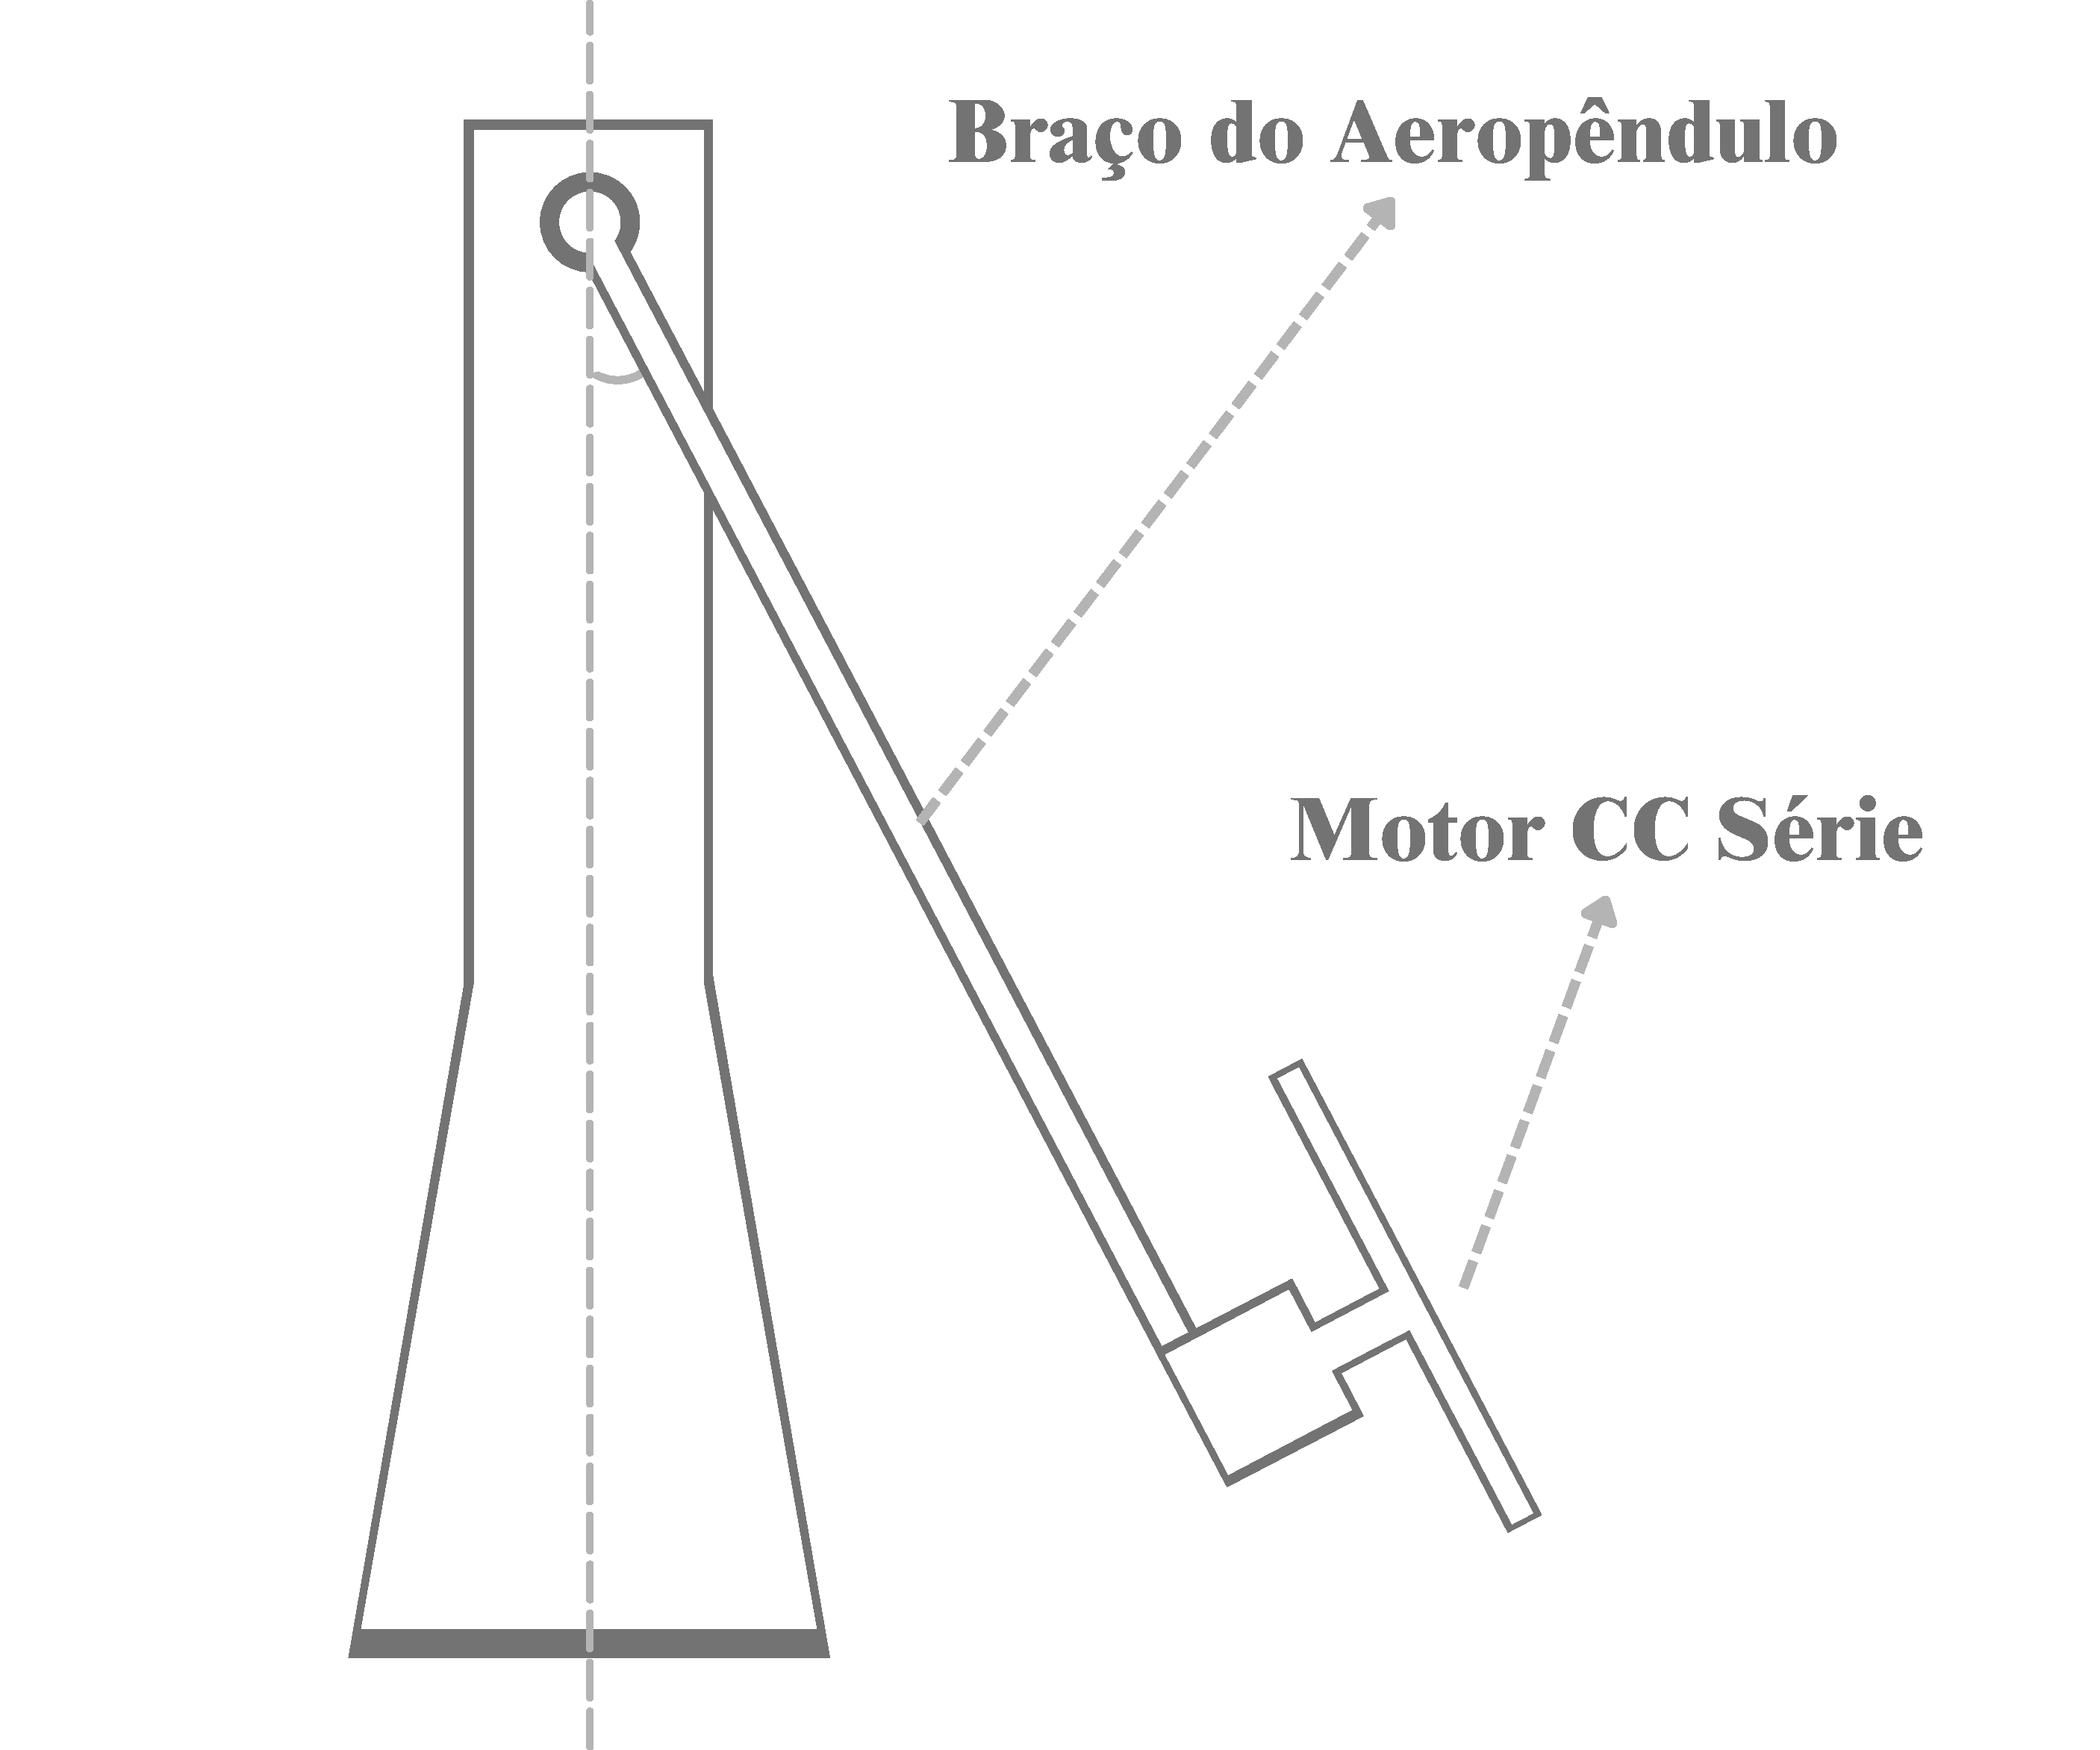
\includegraphics[width=0.55\textwidth]{Capitulos/2_aeropendulo/4_figuras/diagrama_aeropendulo_01.pdf}}
	\caption*{Fonte: elaborado pelo autor (2023).}
        \label{fig4:image_04}
\end{figure}




\section{ Fundamentação Teórica}
\label{fundamentacao_teorica}

O processo que envolve modelagem de sistemas físicos em termos de equações matemáticas é uma das partes mais importante no estudo de sistemas de controle. Segundo \citeonline[p.~11]{ogata5ed}, o modelo matemático de um sistema dinâmico é definido como um conjunto de equações que representa a dinâmica do sistema com precisão ou, pelo menos, razoavelmente bem.

A construção de modelos matemáticos adequados é fundamental na análise de sistemas de controle, pois a dinâmica de diversos sistemas, como mecânicos, elétricos, térmicos, econômicos, biológicos, entre outros, pode ser expressa por meio de equações diferenciais. Tais equações são derivadas das leis físicas que governam cada sistema específico, como as leis de Newton para sistemas mecânicos e as leis de Kirchhoff para sistemas elétricos. Esta abordagem ressalta a importância crucial de compreender as bases matemáticas subjacentes para uma análise abrangente dos sistemas de controle, conforme destacado por \citeonline[p.~11]{ogata5ed}.


% \section{Modelagem Analítica}

Para realizar a modelagem do Aeropêndulo pode-se aplicar diferentes métodos, uma abordagem inicial para modelar sistemas físicos consiste em empregar as leis fundamentais da física. Além disso, em situações mais complexas, é viável decompor o sistema em subsistemas menores e, em seguida, desenvolver modelos para cada um deles. Por fim, é possível conectar esses modelos, de forma a obter uma representação aproximada do sistema real. Dessa maneira, podemos obter uma compreensão mais aprofundada e abrangente da dinâmica do sistema em questão. A figura \ref{fig4:image_01} mostra um diagrama da representação do Aeropêndulo como um conjunto de subsistemas.


\begin{figure}[!h]
	\centering
	\caption{Subsistemas do  Aeropêndulo.}
            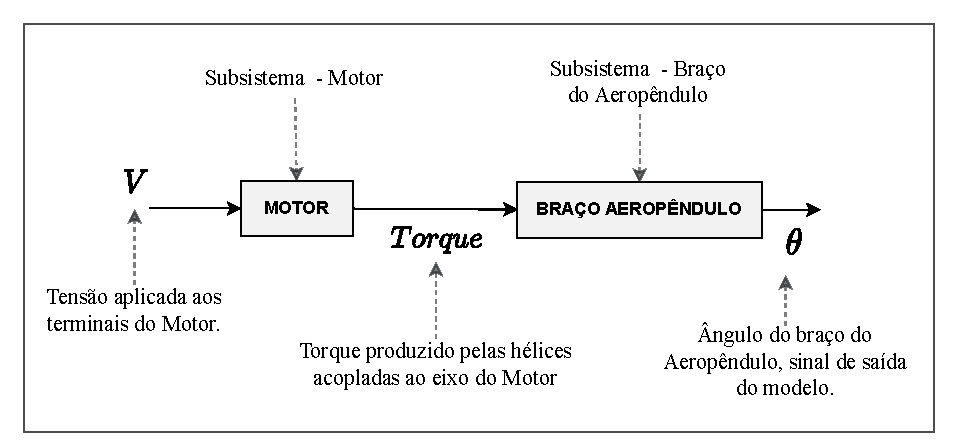
\includegraphics[width=0.9\textwidth]{Capitulos/2_aeropendulo/4_figuras/subsistemas_aeropendulo.pdf}
	\caption*{Fonte: elaborado pelo autor (2023).}
        \label{fig4:image_01}
\end{figure}



\newpage

\subsection{ Modelo Matemático Braço do Aeropêndulo}
\label{modelagem_braco_aeropendulo}

Como previamente abordado, é possível segmentar o sistema em dois subsistemas distintos: o motor CC Série e o braço do Aeropêndulo. Nesta seção, o foco estará concentrado na modelagem do braço do Aeropêndulo, utilizando como referência o trabalho de \cite{amin} para a obtenção da equação que descreve a dinâmica desse componente.


\begin{figure}[!h]
	\centering
	\caption{Diagrama esquemático do Braço do Aeropêndulo.}
	\efbox{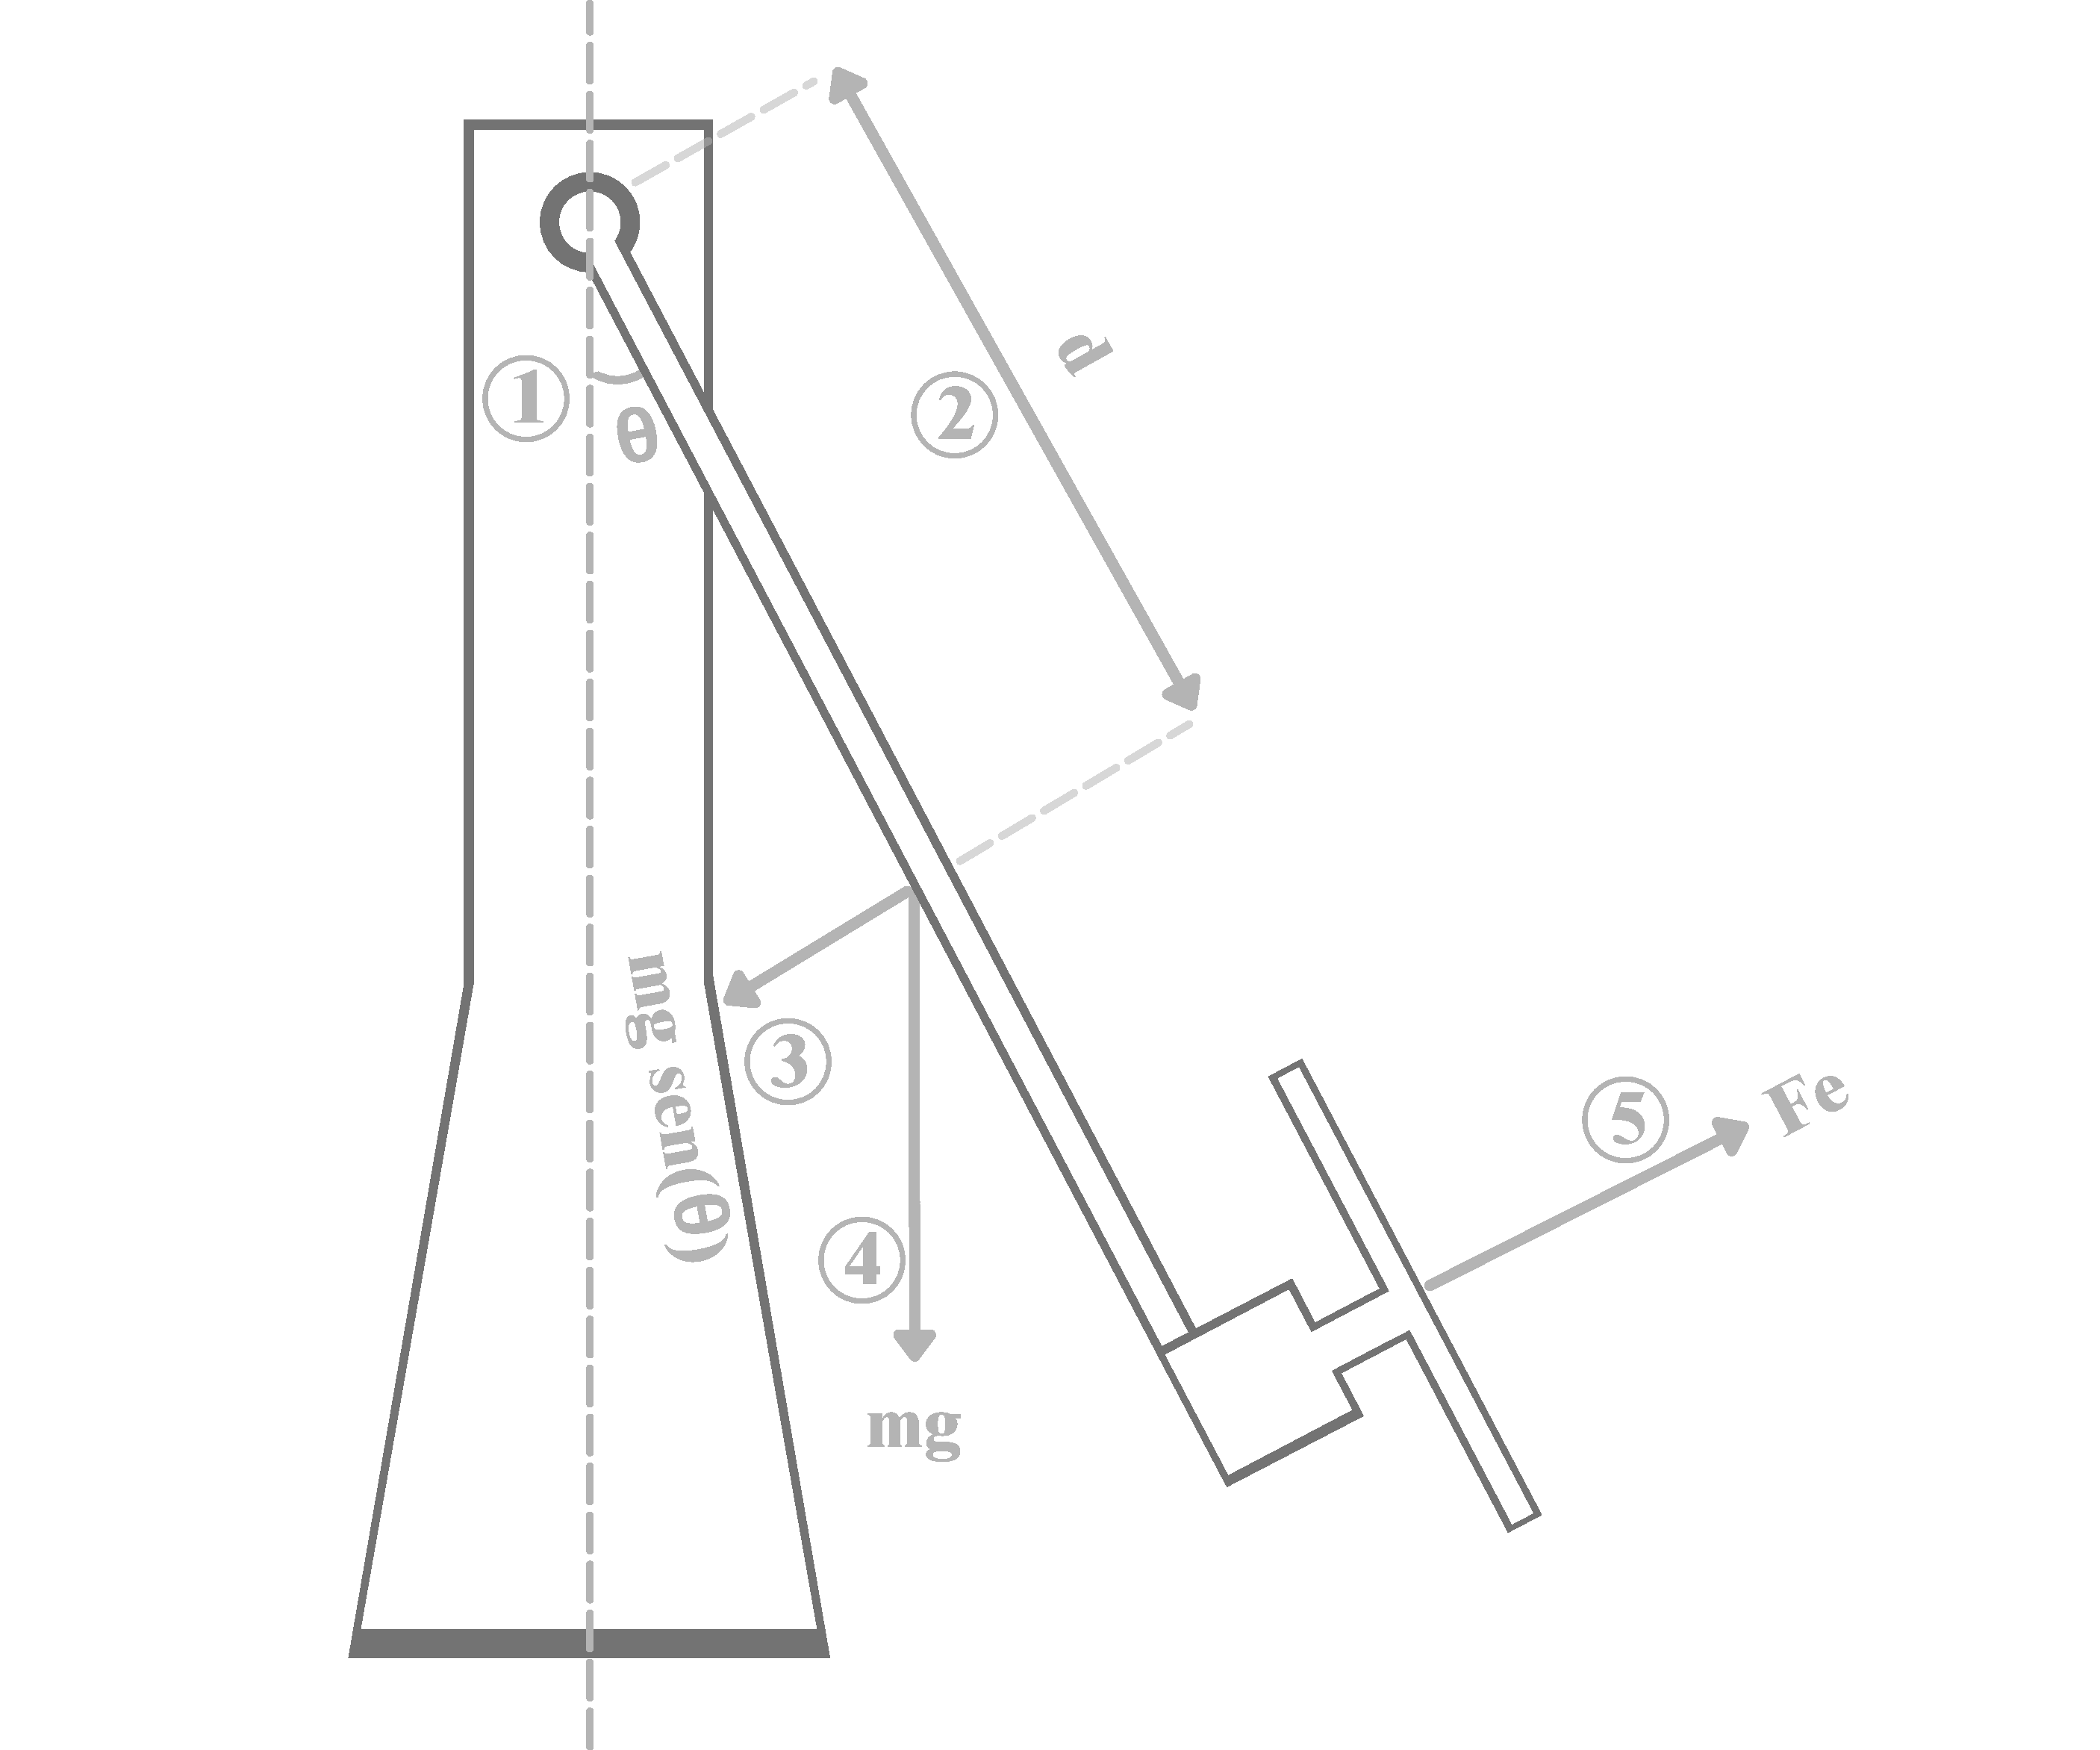
\includegraphics[width=0.55\textwidth]{Capitulos/2_aeropendulo/4_figuras/desenho_aeropendulo.pdf}}
	\caption*{Fonte: elaborado pelo autor (2023).}
        \label{fig4:image_04}
\end{figure}


O modelo matemático do braço do Aeropêndulo é derivado a partir das leis de Newton e do momento angular, como mostra \cite{amin}. assim, se obtém a equação \ref{eq4:eq38}.

\begin{align}
    F_e &= J_b\ddot{\theta} + c\dot{\theta} +mgd\sin{\theta}  \label{eq4:eq38}
\end{align}

\noindent Onde:

\begin{itemize}
        \setlength{\itemsep}{-2pt}
	\item  $F_e$: Empuxo gerado pela hélice
        \item  $J_b$: Momento de inércia do Braço
        \item  $\theta$: posição angular do Aeropêndulo
        \item  $c$: coeficiente de amortecimento viscoso
        \item  $m$: massa do Aeropêndulo
        \item  $d$: a distância entre o centro de massa e o ponto de pivô
\end{itemize}

A entrada do subsistema do braço do Aeropêndulo é a força de empuxo proporcionada pela hélice, porém, o modelo do motor CC Série tem como saída a velocidade angular, dessa forma é preciso encontrar uma relação entre a velocidade $\omega$ e o empuxo $F_e$, essa relação é não linear, $F_e = K_m\omega^2$, porém é possível aproximar por uma relação linear,  $F_e = K_m\omega$, em que $K_m$ é um ganho que relaciona a velocidade angular com o empuxo. Com isso, pode-se relacionar a velocidade angular $\omega$  com o empuxo $F_e$ gerado pela hélice do Aeropêndulo.

O modelo encontrado tem uma parcela não linear dada por $\sin{\theta}$, para aplicar técnicas de projeto de controle é preciso obter o modelo linearizado da planta, isso pode ser feito considerando $\sin{\theta} \approx \theta$ para pequenas variações em torno de $\theta$. dessa forma, temos a seguinte linearização:
\begin{align}
    F_e &= J_b\ddot{\theta} + c\dot{\theta} +mgd\theta
    \label{eq4:eq39}
\end{align}

Aplicando a transformada de Laplace para encontrar a função de transferência do subsistema, tem-se:

\begin{align}
    F_e(s) &= J_b\theta(s)s^2 + c\theta(s)s + mgd\theta(s) \label{eq4:eq41}\\
    F_e(s) &= (J_bs^2 + cs +mgd)\theta(s) \label{eq4:eq42}\\
    \dfrac{\theta(s)}{F_e(s)} &= \frac{1}{J_bs^2 + cs + mgd} \label{eq4:eq43}
\end{align}


Agora que foi obtido o modelo do braço do Aeropêndulo, pode-se usar a relação linearizada $F_e = K_m\omega$ para usar a saída do modelo do motor cc série como entrada do modelo do braço do Aeropêndulo, como mostrado na equação \ref{eq4:eq46}.

\begin{align}
    \dfrac{\theta(s)}{K_m\omega(s)} &= \dfrac{1}{J_bs^2 + cs +mgd} \label{eq4:eq44}\\
    \dfrac{\theta(s)}{\omega(s)} &= \dfrac{K_m}{J_bs^2 + cs +mgd} \label{eq4:eq45}\\
    H(s) = \dfrac{\theta(s)}{\omega(s)} &= \dfrac{\dfrac{K_m}{J_b}}{s^2 + \dfrac{c}{J_b}s +\dfrac{mgd}{J_b}} \label{eq4:eq46}
\end{align}


A equação \ref{eq4:eq46} representa a função de transferência que descreve o comportamento dinâmico do braço do Aeropêndulo. Esta expressão matemática encapsula as relações fundamentais entre as variáveis de entrada/saída do sistema, oferecendo uma visão abrangente e quantitativa da resposta do braço às diferentes condições e estímulos. Ao analisar a função de transferência, podemos compreender como as mudanças nas entradas afetam as saídas.


\subsection{Modelo Matemático do Motor CC Série}
\label{modelagem_motorccserie}

Os motores CC série tem como principal característica possuir o enrolamento de campo em série com o enrolamento de armadora, essa configuração resulta em um motor com torque de partida alto, porém, o torque reduz a medida que a velocidade aumenta devido ao aumento da Força Eletromotriz FEM. Por conta desse aumento de FEM os motores CC Séries tem uma regulação de velocidade ruim, quando se aumenta a carga no eixo do motor a velocidade é reduzida que por sua vez reduz a FEM e então o torque aumenta para conseguir atuar na carga.


No contexto dos motores série, observamos que o aumento da carga resulta em incrementos na corrente, na Força Magnetomotriz (FMM) da armadura e no fluxo do campo do estator, contanto que o ferro não atinja a saturação completa. À medida que o fluxo aumenta com a carga, a velocidade do motor série deve diminuir para manter um equilíbrio adequado entre a tensão aplicada e a força contraeletromotriz. Além disso, o aumento na corrente de armadura, ocasionado pelo acréscimo no conjugado, é menor em comparação com o motor em derivação, devido ao aumento no fluxo. Dessa forma, o motor série é caracterizado como um motor de velocidade variável \citeonline[p.~410]{umans2014}.


No entanto, mesmo motores cc série com dimensões reduzidas geram torques altos com baixo consumo de corrente. Visando melhorar seu desempenho, é possível projetar controladores de malha fechada capazes de tornar esses motores mais eficientes na regulação de velocidade.

Para realizar a modelagem o motor CC série, foi usado a base teórica de \cite{jesus}, A figura \ref{fig4:image_02} mostra um diagrama da configuração do motor CC Série, no qual o enrolamento de campo está conectado em série com o enrolamento de armadura, dessa forma, a  corrente de campo é igual a corrente de armadura $ i = i_f = i_a$.


\begin{figure}[!h]
	\centering
	\caption{Motor CC Série.}
	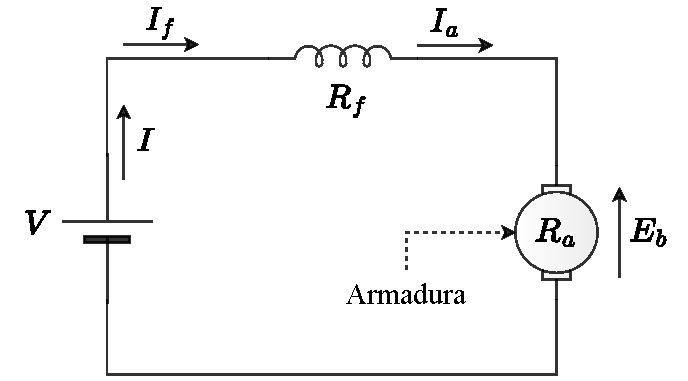
\includegraphics[width=0.7\textwidth]{Capitulos/2_aeropendulo/4_figuras/esquema_motor_cc.pdf}
	\caption*{Fonte:  elaborado pelo autor (2023).}
	\label{fig4:image_02}
\end{figure}

Na figura \ref{fig4:image_03}, mostra o diagrama eletromecânico do motor, nele pode-se observar que os componentes elétricos estão todos em série, no qual o enrolamento de campo possui uma parte resistiva e outra indutiva, assim como o enrolamento de armadura, já a parte mecânica possui uma velocidade angular dada por $\omega$, torque eletromagnético do motor dado por $T_e$ e torque da Carga $T_c$.


\begin{figure}[!h]
	\centering
	\caption{Diagrama Elétrico/Mecânico Motor CC Série.}
	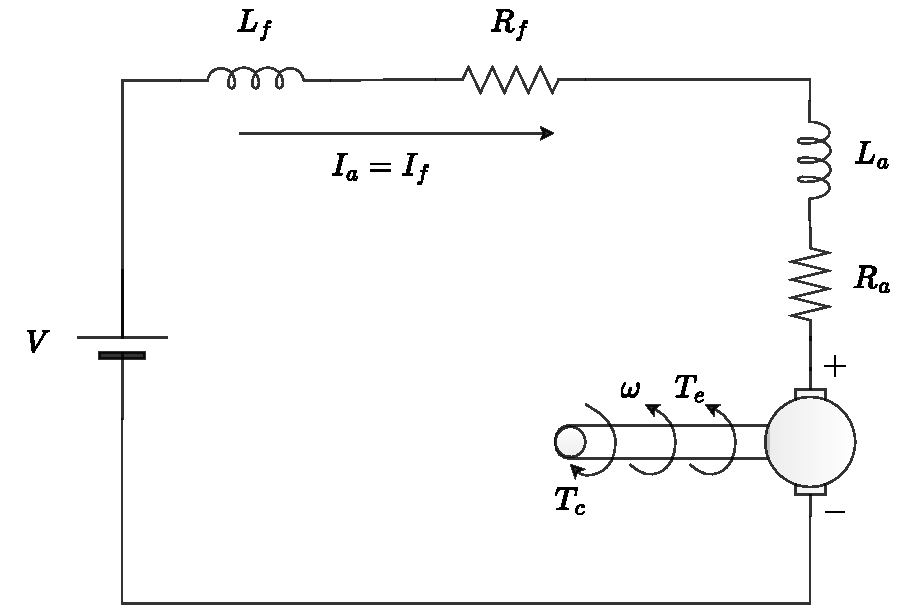
\includegraphics[width=0.6\textwidth]{Capitulos/2_aeropendulo/4_figuras/diagrama_motor_cc.pdf}
	\caption*{Fonte: elaborado pelo autor (2023).}
	\label{fig4:image_03}
\end{figure}


%%%%%%%%%%%%%%%%%%%%%%%%%%%%%%%%%%%%%%%%%%%%%%%%%%%%%%%%%%%%%%%%%%%%%%%%%%%%%%%%%%%%%%%%%%%%%%%%%%%%%%%%%%%%%%%%%%%%%%%%%%%%%%%%%%%%%%%%%
%%%%%%%%%%%%%%%%%%%%%%%%%%%%%%%%%%%%%%%%%%%%% Modelagem da Parte Mecânica do Motor CC Série %%%%%%%%%%%%%%%%%%%%%%%%%%%%%%%%%%%%%%%%%%%%%
%%%%%%%%%%%%%%%%%%%%%%%%%%%%%%%%%%%%%%%%%%%%%%%%%%%%%%%%%%%%%%%%%%%%%%%%%%%%%%%%%%%%%%%%%%%%%%%%%%%%%%%%%%%%%%%%%%%%%%%%%%%%%%%%%%%%%%%%%

%\subsubsection{Modelagem da Parte Mecânica do Motor CC Série}

Primeiramente a parte mecânica do motor será modelada, um motor cc série é composto por uma parte rotativa "armadura", de modo que, essa parte, gera um momento de inércia $J_m$ no eixo do motor e um fator de amortecimento viscoso $b$, além disso, o eixo possui uma velocidade angular $\dot{\omega}$.

Assim, a equação \ref{eq4:eq1}, obtida a partir de \cite{jesus}, descreve o modelo mecânico do motor CC Série.

\begin{align}
	J_m\ddot{\omega}(t) &= T_e(t) - b\dot{\omega}(t) - T_c(t) \label{eq4:eq1}
\end{align}


Ao expressar o torque $T_e(t)$ em função das outras variáveis, obtém-se a equação \ref{eq4:eq2}.

\begin{align}
	T_e(t) &= J_m\ddot{\omega}(t) + b\dot{\omega}(t) + T_c(t) \label{eq4:eq2}
\end{align}


\noindent Onde:
\begin{itemize}
        \setlength{\itemsep}{-2pt}
	\item $T_e$: Torque Eletromagnético produzido pelo Motor;
	\item $J_m$: Momento de Inércia do Eixo do Motor;
	\item $\ddot{\omega}$: Aceleração Angular do Eixo do Motor;
	\item $\dot{\omega}$: Velocidade Angular do Eixo do Motor;
	\item $b$: Fator de Amortecimento Viscoso;
	\item $T_c$: Torque de Carga.
\end{itemize}

Tanto a Força Eletromotriz $E_A(t)$ quanto o Torque Eletromagnético $T_e(t)$ dependem do fluxo magnético do entreferro $\Phi$, com isso, tem-se as equações \ref{eq4:eq3} e \ref{eq4:eq4}.

\begin{align}
	E_a(t) &= \dot{\omega}(t) \Phi{(i)} \label{eq4:eq3}\\
	T_e(t) &= i(t) \Phi{(i)}			\label{eq4:eq4}
\end{align}

O Fluxo magnético depende da corrente $i(t)$, assim, as equações \ref{eq4:eq1} e \ref{eq4:eq2} são não-lineares. Além disso, pode-se aproximar o fluxo $\Phi$ por uma relação linear, $K_0$, ao desprezar a saturação magnética.

\begin{align}
	\Phi(i) &= K_0 i(t) \label{eq4:eq5}
\end{align}

A constante $K_0$ é a indutância mútua entre a armadura e o enrolamento de campo. Agora pode-se encontrar o modelo não-linear da parte mecânica do Motor CC Série, substituindo \ref{eq4:eq5} em \ref{eq4:eq4}, obtém-se a expressão \ref{eq4:eq7}:

\begin{align}
	T_e(t) &= i(t) K_0 i(t) \label{eq4:eq6}\\
	T_e(t) &= K_0 i^2(t) 	\label{eq4:eq7}
\end{align}

Substituindo \ref{eq4:eq7} em \ref{eq4:eq2}, é possível encontrar o modelo da parte mecânica do motor CC série, assim, tem-se a expressão  \ref{eq4:eq8}.


\begin{align}
	K_0 i^2(t) &= J_m\ddot{\omega}(t) + b\dot{\omega}(t) + T_c(t) \label{eq4:eq8}
\end{align}


%%%%%%%%%%%%%%%%%%%%%%%%%%%%%%%%%%%%%%%%%%%%%%%%%%%%%%%%%%%%%%%%%%%%%%%%%%%%%%%%%%%%%%%%%%%%%%%%%%%%%%%%%%%%%%%%%%%%%%%%%%%%%%%%%%%%%%%%%
%%%%%%%%%%%%%%%%%%%%%%%%%%%%%%%%%%%%%%%%%%%%% Modelagem da Parte Elétrica do Motor CC Série %%%%%%%%%%%%%%%%%%%%%%%%%%%%%%%%%%%%%%%%%%%%%
%%%%%%%%%%%%%%%%%%%%%%%%%%%%%%%%%%%%%%%%%%%%%%%%%%%%%%%%%%%%%%%%%%%%%%%%%%%%%%%%%%%%%%%%%%%%%%%%%%%%%%%%%%%%%%%%%%%%%%%%%%%%%%%%%%%%%%%%%

% \subsubsection{Modelagem da Parte Elétrica do Motor CC Série}

Para a parte elétrica, utilizou-se a lei de Kirchhoff das tensões para modelar o sistema. assim como a parte mecânica, o modelo da parte elétrica foi baseado de \cite{jesus}, o motor em questão é um motor de corrente contínua CC série, Dessa forma, $i_a = i_f$, portanto, obtém-se a expressão \ref{eq4:eq9}.


\begin{align}
	V(t) &= (R_a + R_f)i(t)+ (L_a + L_f)\dfrac{d}{dt}i(t) + E_a \label{eq4:eq9}
\end{align}

\noindent Onde:

\begin{itemize}
        \setlength{\itemsep}{-2pt}
	\item $V$: Tensão da Fonte;
	\item $R_a$: Resistência da Armadura;
	\item $R_f$: Resistência de Campo;
	\item $i_a$: Corrente da Armadura;
	\item $i_f$: Corrente de Campo;
	\item $E_A$: Tensão Contro Eletromotriz Gerada pela Armadura;
	\item $L_a$: Impedância da Armadura;
	\item $L_f$: Impedância de Campo.
\end{itemize}

Como os componentes elétricos então em série, pode-se obter uma resistência total assim como uma indutância:

\begin{align}
	R &= R_a + R_f          \label{eq4:eq10}\\        
	L &= L_a + L_f          \label{eq4:eq11}
\end{align}

\begin{align}
	V(t) &= Ri(t)+ L\dfrac{d}{dt}i(t) + E_a \label{eq4:eq12}
\end{align}

Substituindo \ref{eq4:eq5} em \ref{eq4:eq3}, obtém-se a equação \ref{eq4:eq13}.

\begin{align}
	E_a(t) &= \dot{\omega}(t)K_0 i(t) \label{eq4:eq13}
\end{align}

Por fim, pode-se encontrar a equação que descreve a parte elétrica do sistema ao substituir \ref{eq4:eq13} em \ref{eq4:eq12}, assim, obtendo a equação \ref{eq4:eq14}.

\begin{align}
	V(t) &= Ri(t)+ L\frac{d}{dt}i(t) + \dot{\omega}(t)K_0 i(t) \label{eq4:eq14}
\end{align}

Dessa forma, as equações que modelam um Motor CC série são expressas por \ref{eq4:eq15} e \ref{eq4:eq16}, em que \ref{eq4:eq15} esta relacionada a parte mecânica e \ref{eq4:eq16} a parte elétrica.

\begin{align}
	K_0 i^2(t) &= J_m\ddot{\omega}(t) + b\dot{\omega}(t) + T_c(t) \label{eq4:eq15}\\
	V(t) &= Ri(t)+ L\dfrac{d}{dt}i(t) + \dot{\omega}(t)K_0 i(t) \label{eq4:eq16}
\end{align}

\vspace{1cm}

\subsubsection{Linearização do modelo do Motor CC Série}

Para projetos de controle lineares é preciso linearizar o modelo encontrado, para isso, vamos reorganizar as equações \ref{eq4:eq15} e \ref{eq4:eq16}, assim obtêm-se as equações \ref{eq4:eq17} e \ref{eq4:eq18}:

\begin{align}
    \ddot{\omega}(t) &= \dfrac{K_0}{J_m} i^2(t) - \frac{b}{J_m}\dot{\omega}(t) - \dfrac{1}{J_m}T_c(t) \label{eq4:eq17}\\
    \dfrac{d}{dt}i(t) &= \dfrac{R}{L}i(t)- \dfrac{K_0}{L}\dot{\omega}(t)i(t) +\dfrac{1}{L}V(t) \label{eq4:eq18}
\end{align}

Reescrevendo as equações de estados na forma matricial,

\begin{align}
    x_1 = \dot{\omega}  \label{eq4:eq19}\\
    x_2 = i   \label{eq4:eq20}
\end{align}


Coeficientes da equação de estado \ref{eq4:eq17}.

\begin{align}
    a_1 = \dfrac{K_0}{J_m}; \quad a_2 = \dfrac{b}{J_m}; \quad a_3 = \dfrac{1}{J_m}  \label{eq4:eq21}
\end{align}

Coeficientes da equação de estado \ref{eq4:eq18}.

\begin{align}
    b_1 = \dfrac{R}{L}; \quad b_2 = \dfrac{K_0}{L}; \quad b_3 = \dfrac{1}{L}  \label{eq4:eq22}
\end{align}

Representação no espaço de estados do motor CC Série não-linear

\begin{align}
    \dot{x}_1 &= a_1x_2^2  - a_2x_1 -a_3T_c   \label{eq4:eq23}\\
    \dot{x}_2 &= -b_1x_2  -b_2x_1x_2 + b_3V    \label{eq4:eq24}
\end{align}



\begin{align}
\dot{x} = \begin{bmatrix}
    \dot{x}_1\\
    \dot{x}_2
\end{bmatrix} = 
\begin{bmatrix}
    a_1x_2^2 -a_2x_1 -a_3T_c \\
    -b_1x_2 -b_2x_1x_2 + b_3V
\end{bmatrix} = f(x, u)  \label{eq4:eq25}
\end{align}

O ponto de equilíbrio $(x_1^0, x_2^0)$ das equações \ref{eq4:eq23} e \ref{eq4:eq24} é encontrado zerando as derivadas, como mostrado em \ref{eq4:eq26} e \ref{eq4:eq27}.


\begin{align}
     x_2^0 &= \sqrt{\frac{a_2x_1^0 + a_3T_c}{a_1}} \label{eq4:eq26}\\
     V &= \frac{x_2^0(b_1+b_2x_1^0)}{b_3} \label{eq4:eq27}
\end{align}


A linearização de  \ref{eq4:eq23} e \ref{eq4:eq24} em torno do ponto de equilíbrio é obtida encontrando o jacobiano das mesmas, assim se obtêm as matrizes $A$ e $B$.

\begin{align}
     \dot{x} &= Ax + Bu    \label{eq4:eq28}\\
     y &= Cx               \label{eq4:eq29}
\end{align}

Em que, 

\begin{align}
     A &= \left. \dfrac{\partial f(x,y)}{\partial x}\right|_{x_1^0, x_2^0} = \begin{bmatrix}
    -a_2       &   2a_1x_2^0\\
    -b_2x_2^0  & -(b_1+b_2x_1^0)
\end{bmatrix}    \label{eq4:eq30}\\
B &= \left. \dfrac{\partial f(x,y)}{\partial u}\right|_{x_1^0, x_2^0} = \begin{bmatrix}
    -a_3       &   0\\
    0  & b_3
\end{bmatrix}    \label{eq4:eq31}\\
C &= [1, 0]      \label{eq4:eq32}\\
\end{align}


Onde,

\begin{align}
    u &= \begin{bmatrix}
        T_c\\
        V
\end{bmatrix}           \label{eq4:eq33}\\
y &= \dot{\omega}(t)    \label{eq4:eq34}
\end{align}


Se o torque de carga for considerado zero, $T_c = 0$, temos as seguintes expressões,

\begin{align}
     x_2^0 = \sqrt{\frac{a_2x_1^0}{a_1}}; \quad
         V = \frac{x_2^0(b_1+b_2x_1^0)}{b_3}; \quad
         B = \begin{bmatrix}
        0\\
        b_3
\end{bmatrix}  \label{eq4:eq35}
\end{align}

Agora é possível encontrar a função de transferência $G(s)$ associada as matrizes de estados $A, B, C$ linearizadas, para isso usa-se a expressão \ref{eq4:eq36}.


\begin{align}
    G(s) &= \frac{\dot{\omega}(s)}{V(s)} = C(sI-A)^{-1}B     \label{eq4:eq36}
\end{align}

Substituindo as matrizes $A$, $B$ e $C$ em \ref{eq4:eq36}, chega-se a expressão \ref{eq4:eq36_1}.

\begin{align}
    G(s) &= \frac{\dot{\omega}(s)}{V(s)} = \begin{bmatrix}
        1 & 0
\end{bmatrix} \cdot \left(s \cdot \begin{bmatrix}
    1  & 0\\
    0  & 1
\end{bmatrix}-\begin{bmatrix}
    -a_2       &   2a_1x_2^0\\
    -b_2x_2^0  & -(b_1+b_2x_1^0)
\end{bmatrix}\right)^{-1} \cdot \begin{bmatrix}
    -a_3       &   0\\
    0  & b_3
\end{bmatrix}     \label{eq4:eq36_1}
\end{align}

Assim, obtém-se a função de transferência linearizada em função dos parâmetros do motor CC Série, como mostra a equação \ref{eq4:eq37}.



\begin{align}
    G(s) &= \frac{\dot{\omega}(s)}{V(s)} = \dfrac{2 K_{0} \sqrt{\dfrac{b x^{0}_{1}}{K_{0}}}}{J_m L s^{2} + \left(J_m K_{0} x^{0}_{1} + J_m R + L b\right)s  + 3 K_{0} b x^{0}_{1} + R b }     \label{eq4:eq37}
\end{align}

\vspace{1cm}



%\vspace{1cm}
\subsection{Junção dos subsistemas}
\label{junca0_submodelos}

A partir dos modelos encontrados nas subseções \ref{modelagem_motorccserie} e \ref{modelagem_braco_aeropendulo} pode-se obter o modelo completo do sistema unindo os subsistemas como mostra a figura \ref{fig4:image_05}. com isso, é possível modelar o Aeropêndulo tendo como entrada a tensão no motor CC série e como saída o ângulo do braço.

\begin{figure}[!h]
	\centering
	\caption{Diagrama da junção dos subsistemas do  Aeropêndulo.}
            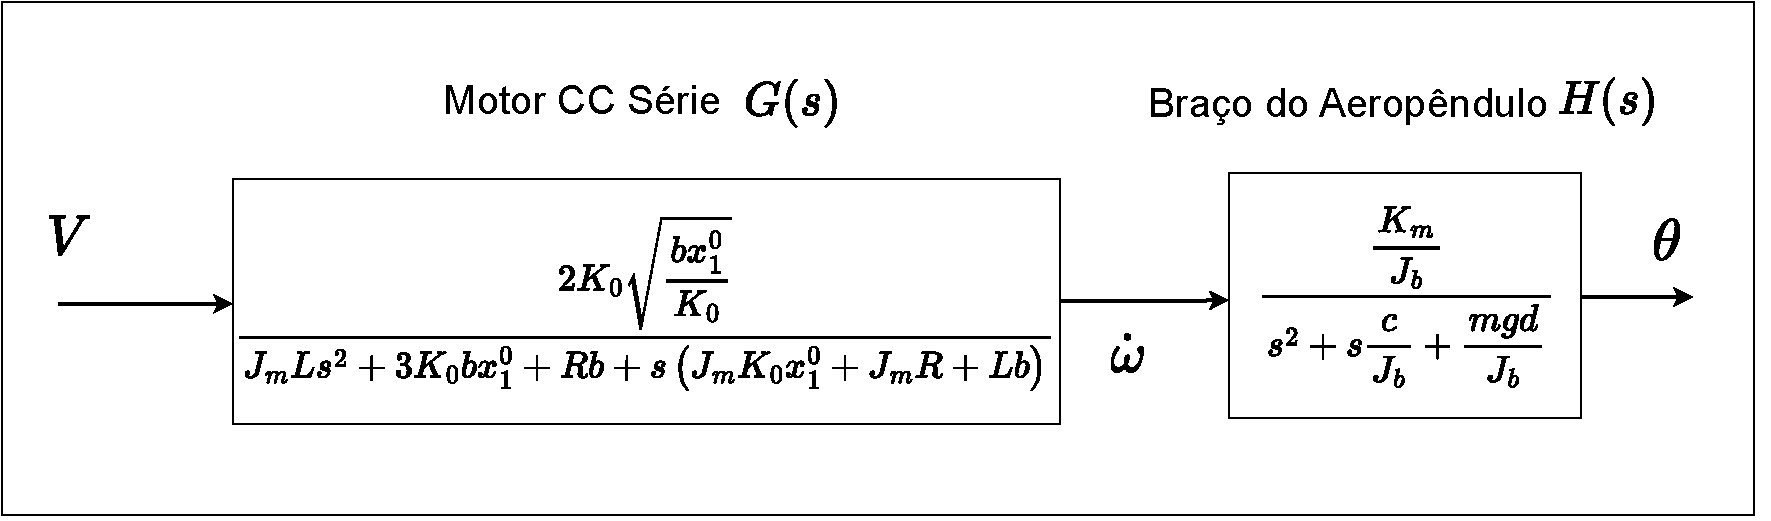
\includegraphics[width=1\textwidth, page=1]{Capitulos/2_aeropendulo/4_figuras/ft_subsistemas.pdf}
	\caption*{Fonte: elaborado pelo autor (2023).}
        \label{fig4:image_05}
\end{figure}



A modelagem usando as leis físicas permite uma interpretação dos parâmetros da planta e ajuda a entender a influência deles na dinâmica do sistema, no entanto, ao utilizar esse método de modelagem surgi uma complexidade em obter os valores numéricos de alguns desses parâmetros, por exemplo, o Momento de Inércia do Eixo do Motor $J_m$ se torna complicado de se obter, assim como o Coeficiente de Amortecimento Viscoso $c$ do pivô do braço do Aeropêndulo entre outros parâmetros, com isso, surgi um método alternativo que permite modela um sistema usando dados de ensaios chamado de Identificação de Sistema, esse método usando os dados de entrada e saída e aproxima um modelo, com isso se obtêm uma função de transferência discreta.

% \section{Modelagem por Identificação de Sistemas}
%\label{model_ident_sis}
%Segundo \cite{aguirre2004intro}, A identificação de sistemas se propõe a obter um modelo matemático que explique, pelo menos em parte e de forma aproximada, a relação de causa e efeito presente nos dados. Isso permite ter uma relação entrada/saída, em que é determinada por meio de uma equação.

CONTINUA ...

%#############################################################################

\newpage
%\section{Implementação do Protótipo}
%\label{implementacao_prototipo}

\subsection{Protótipo Aeropêndulo}
O projeto para o desenvolvimento do protótipo consiste em uma estrutura mecânica e componentes eletrônicos, a Figura \ref{fig3:image_01} mostra o protótipo finalizado com a parte estrutural e elétrica montada.


\begin{figure}[!h]
	\centering
	\caption{Protótipo do Aeropêndulo.}
	\efbox{\includegraphics[width=0.9\textwidth]{Capitulos/3_hardware_softwares/3_figuras/prot_final.pdf}}
	\caption*{Fonte: elaborado pelo autor (2023).}
	\label{fig3:image_01}
\end{figure}


\subsection{ Parte estrutural do sistema}

 O material escolhido para a estrutura foi o compensado, as chapas de compensado são materiais versáteis e amplamente utilizados na indústria da construção, marcenaria e artesanato. Elas são fabricadas a partir de finas lâminas de madeira, conhecidas como lâminas de folheado, coladas umas sobre as outras com fibras perpendiculares, conferindo maior estabilidade e resistência mecânica ao produto final, Figura \ref{fig3:image_02}.


\begin{figure}[!h]
	\centering
	\caption{Chapas de compensado.}
	\efbox{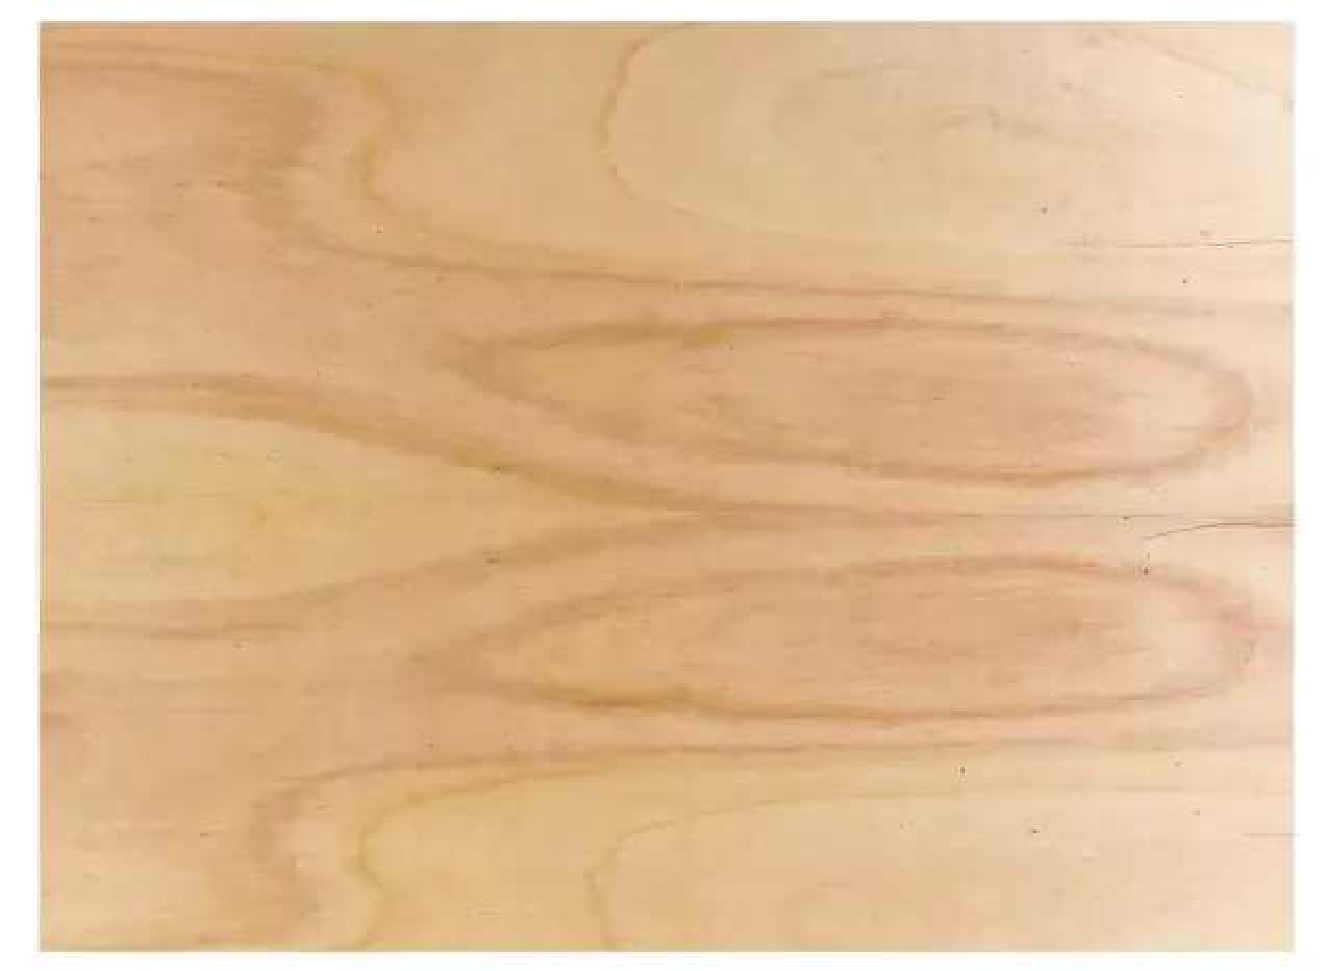
\includegraphics[width=0.6\textwidth]{Capitulos/3_hardware_softwares/3_figuras/compensado.pdf}}
	\caption*{Fonte: elaborado pelo autor (2023).}
	\label{fig3:image_02}
\end{figure}

\newpage
 Já para o braço do Aeropêndulo foi usando Tubo de Fibra de Vidro de Carbono 3x3x2mm, Figura \ref{fig3:image_03}, este material destaca-se por sua leveza e resistência física. No caso do braço do Aeropêndulo, localizado em sua extremidade, há um conjunto motor/hélice encarregado de impulsionar a dinâmica do sistema. Para otimizar o desempenho, é essencial minimizar a massa do braço. Ao fazer isso, as forças de resistência enfrentadas pela força de empuxo serão reduzidas, resultando em uma dinâmica mais ágil e eficiente do sistema.

\begin{figure}[!h]
	\centering
	\caption{Tubo de Fibra de Vidro de Carbono 3x3x2mm.}
	\efbox{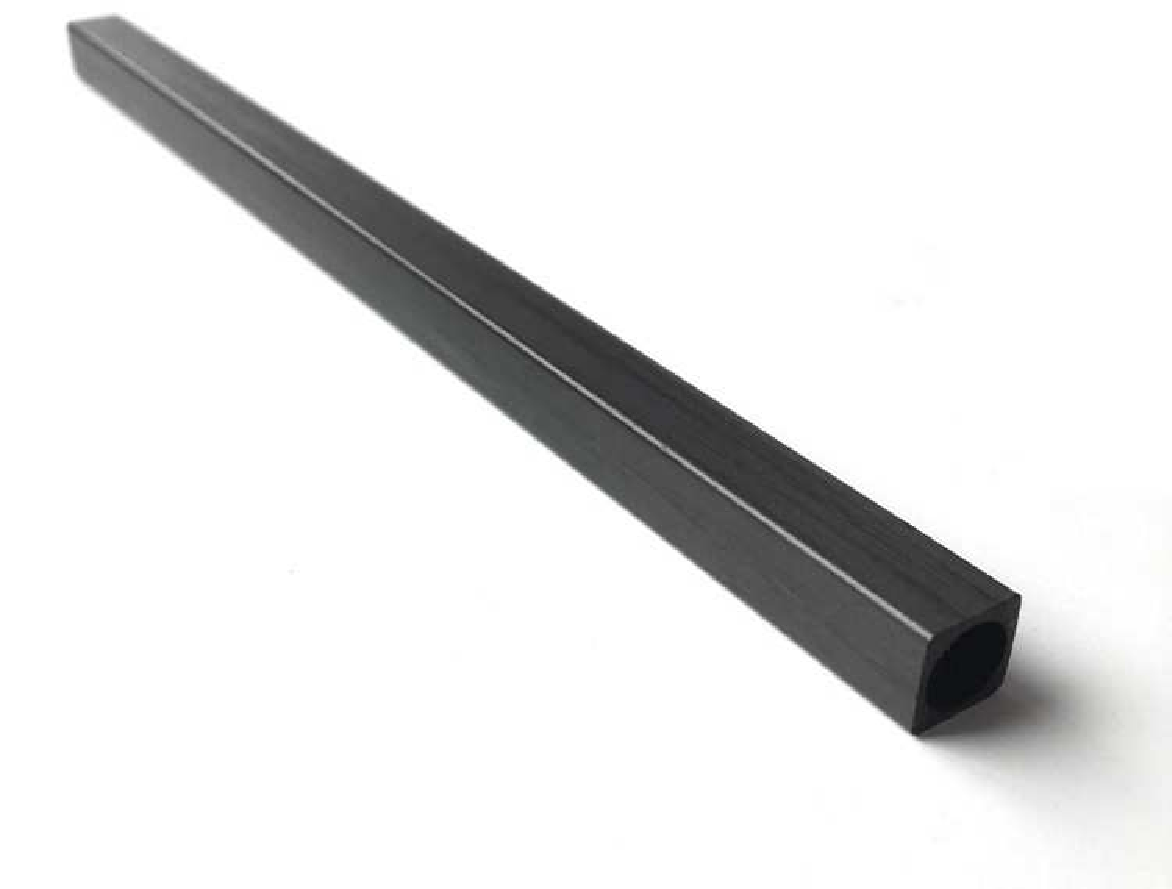
\includegraphics[width=0.5\textwidth]{Capitulos/3_hardware_softwares/3_figuras/carbono2x2mm.pdf}}
	\caption*{Fonte: elaborado pelo autor (2023).}
	\label{fig3:image_03}
\end{figure}


\subsection{Parte Elétrica do sistema}

Foram empregados os seguintes componentes eletrônicos no projeto: um Potenciômetro $50k\Omega$, uma Placa de desenvolvimento Esp32, um Módulo Driver L298n, um Conjunto (suporte/motor/hélice para drones fpv racing quadcopter) e componentes eletrônicos (resistor, capacitor).

\subsubsection{Potenciômetro $50k\Omega$}

O potenciômetro, Figura \ref{fig3:image_04}, desempenha o papel de \textit{encoder} ao obter o ângulo de inclinação do braço do Aeropêndulo. Essa funcionalidade é viabilizada pelo fato de que, conforme o braço se movimenta, a resistência do potenciômetro se altera, resultando em uma variação na tensão registrada em seus terminais. Essa interação permite estabelecer uma correlação entre a mudança na tensão elétrica e o ângulo de inclinação do braço do Aeropêndulo de maneira precisa e controlada.

\begin{figure}[!h]
	\centering
	\caption{Potenciômetro $50k\Omega$.}
	\efbox{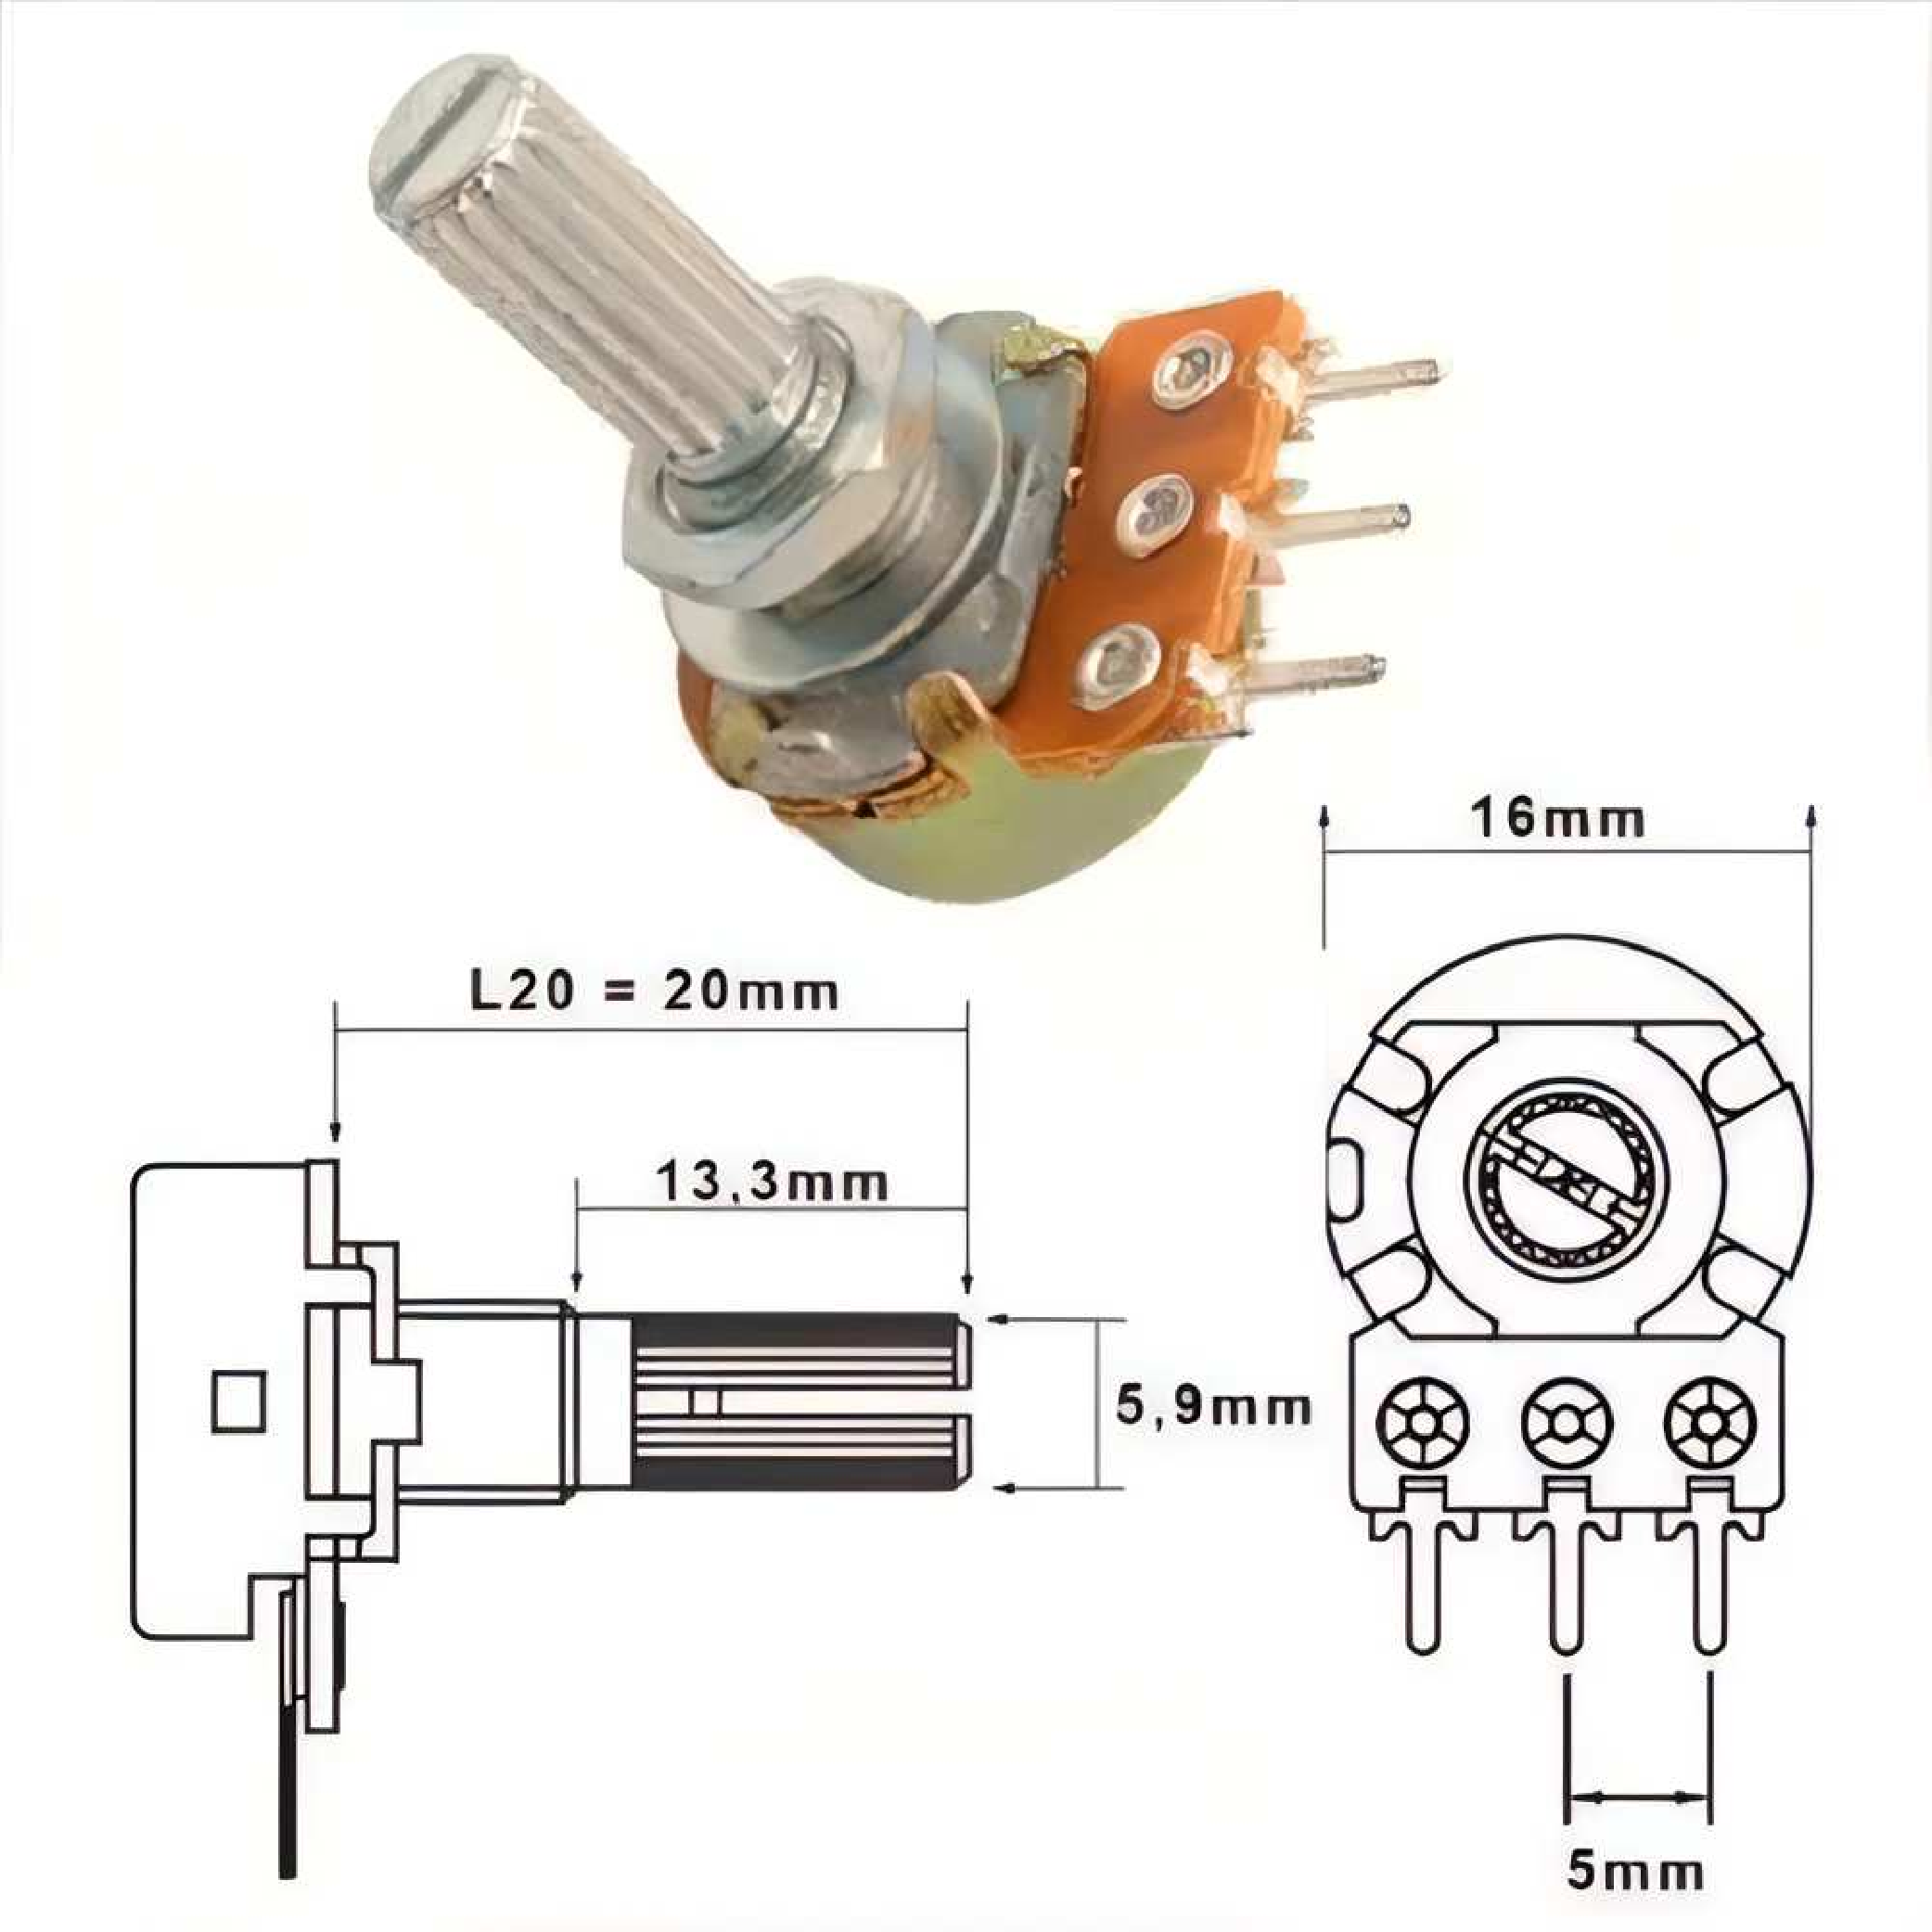
\includegraphics[width=0.5\textwidth]{Capitulos/3_hardware_softwares/3_figuras/pote.pdf}}
	\caption*{Fonte: elaborado pelo autor (2023).}
	\label{fig3:image_04}
\end{figure}




\subsubsection{Placa de desenvolvimento Esp32}

A placa de desenvolvimento ESP32 é uma poderosa e versátil plataforma que integra o popular microcontrolador ESP32 desenvolvido pela empresa  \textit{Espressif}. Projetada para atender às demandas de projetos de Internet das Coisas (IoT) e aplicações de conectividade sem fio, a ESP32 oferece uma vasta gama de recursos e funcionalidades. Equipada com um processador dual-core de 32 bits, Wi-Fi, Bluetooth, interfaces GPIO, I2C, SPI e UART, bem como suporte para memória externa.

A placa desempenhará uma função central no projeto, servindo tanto para a implementação do controlador discreto quanto para a obtenção de dados em tempo real relacionados aos estados do sistema. Esses estados incluem a leitura do sensor de ângulo do braço, a aquisição do sinal de controle e o cálculo do sinal de erro. Adicionalmente, a placa será empregada na geração dos sinais de referência necessários para o funcionamento ideal do sistema, A figura \ref{fig3:image_05} ilustra a placa de desenvolvimento Esp32.

\begin{figure}[!h]
	\centering
	\caption{Placa de desenvolvimento Esp32.}
	\efbox{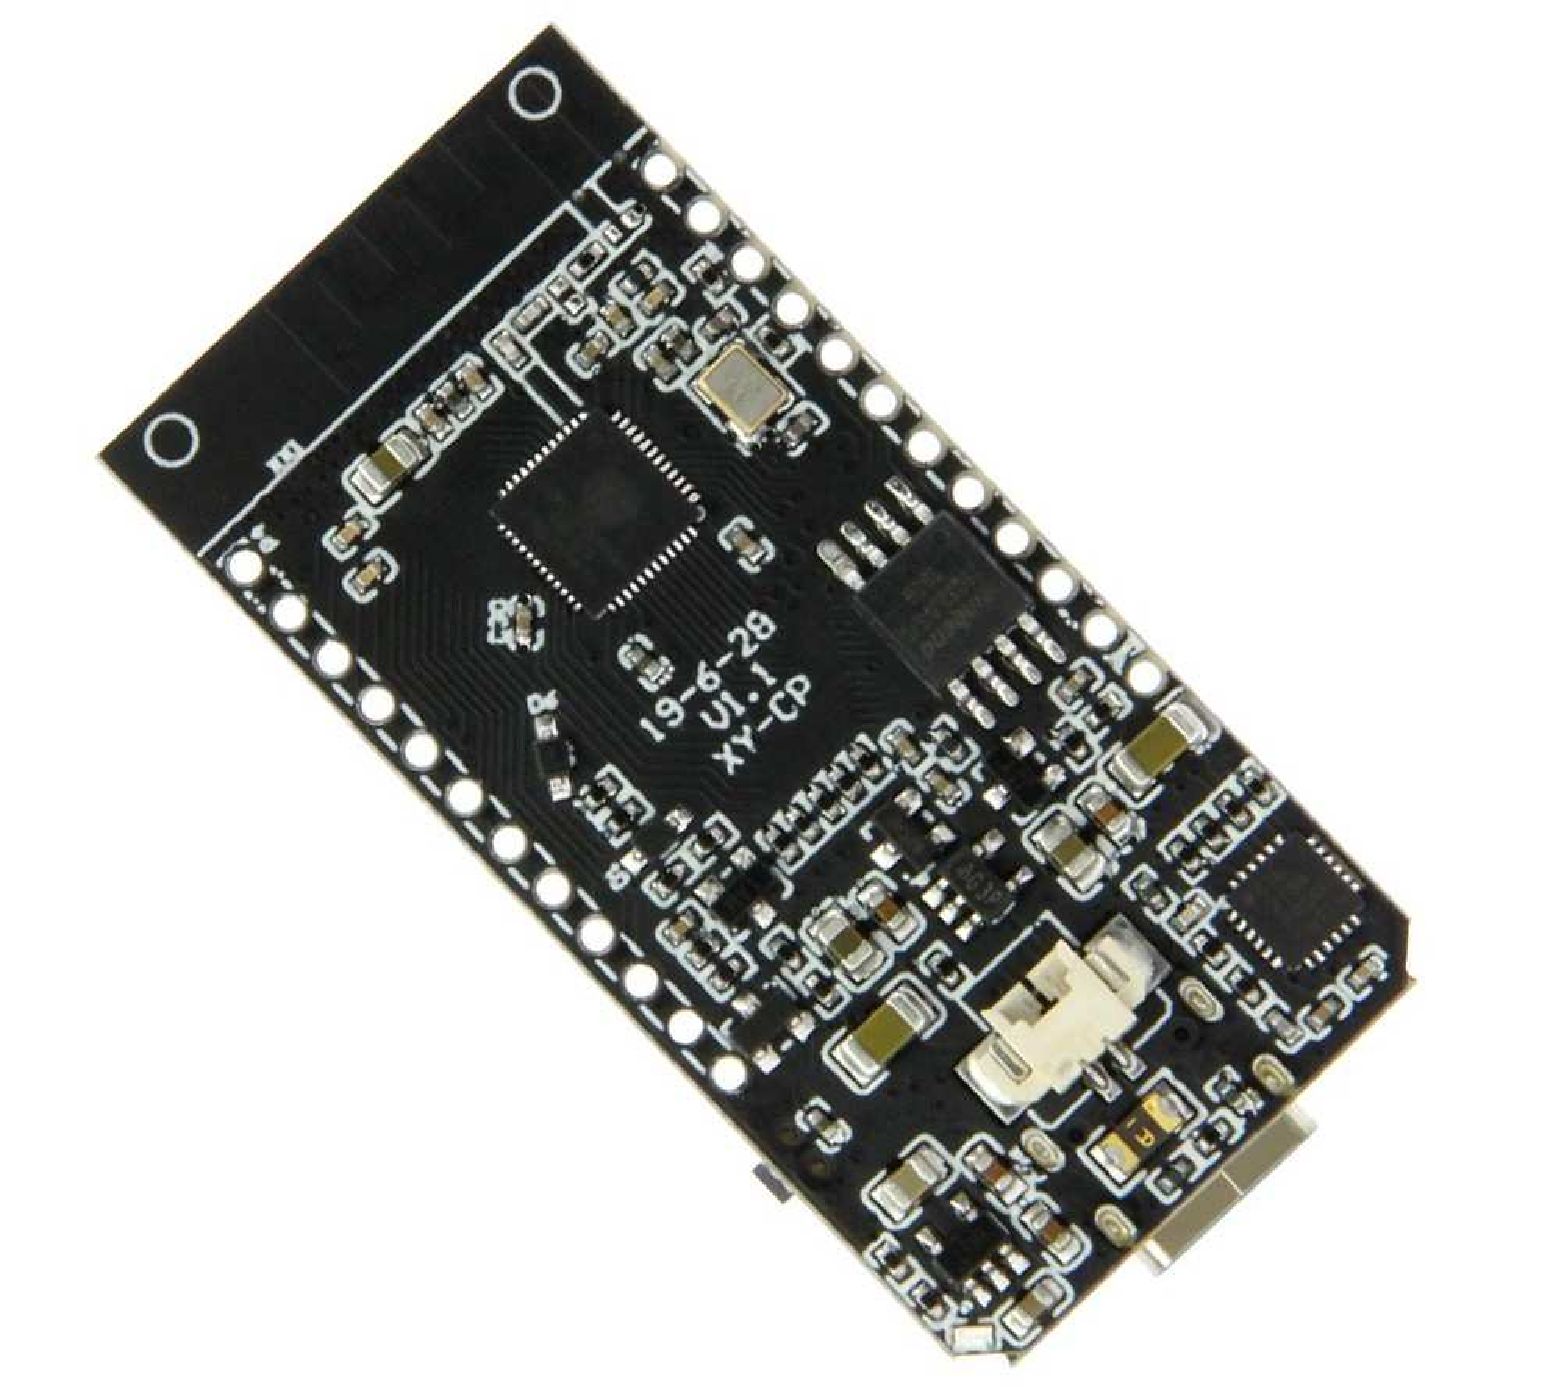
\includegraphics[width=0.5\textwidth]{Capitulos/3_hardware_softwares/3_figuras/f1_esp32.pdf}}
	\caption*{Fonte: elaborado pelo autor (2023).}
	\label{fig3:image_05}
\end{figure}


\subsubsection{Fonte Chaveada 2A, 5V, 25W}

Para a alimentação do motor CC série, foi usado uma fonte de alimentação de 5V/5A, Figura \ref{fig3:image_06}.

\begin{figure}[!h]
	\centering
	\caption{Fonte Chaveada 2A, 5V, 25W.}
	\efbox{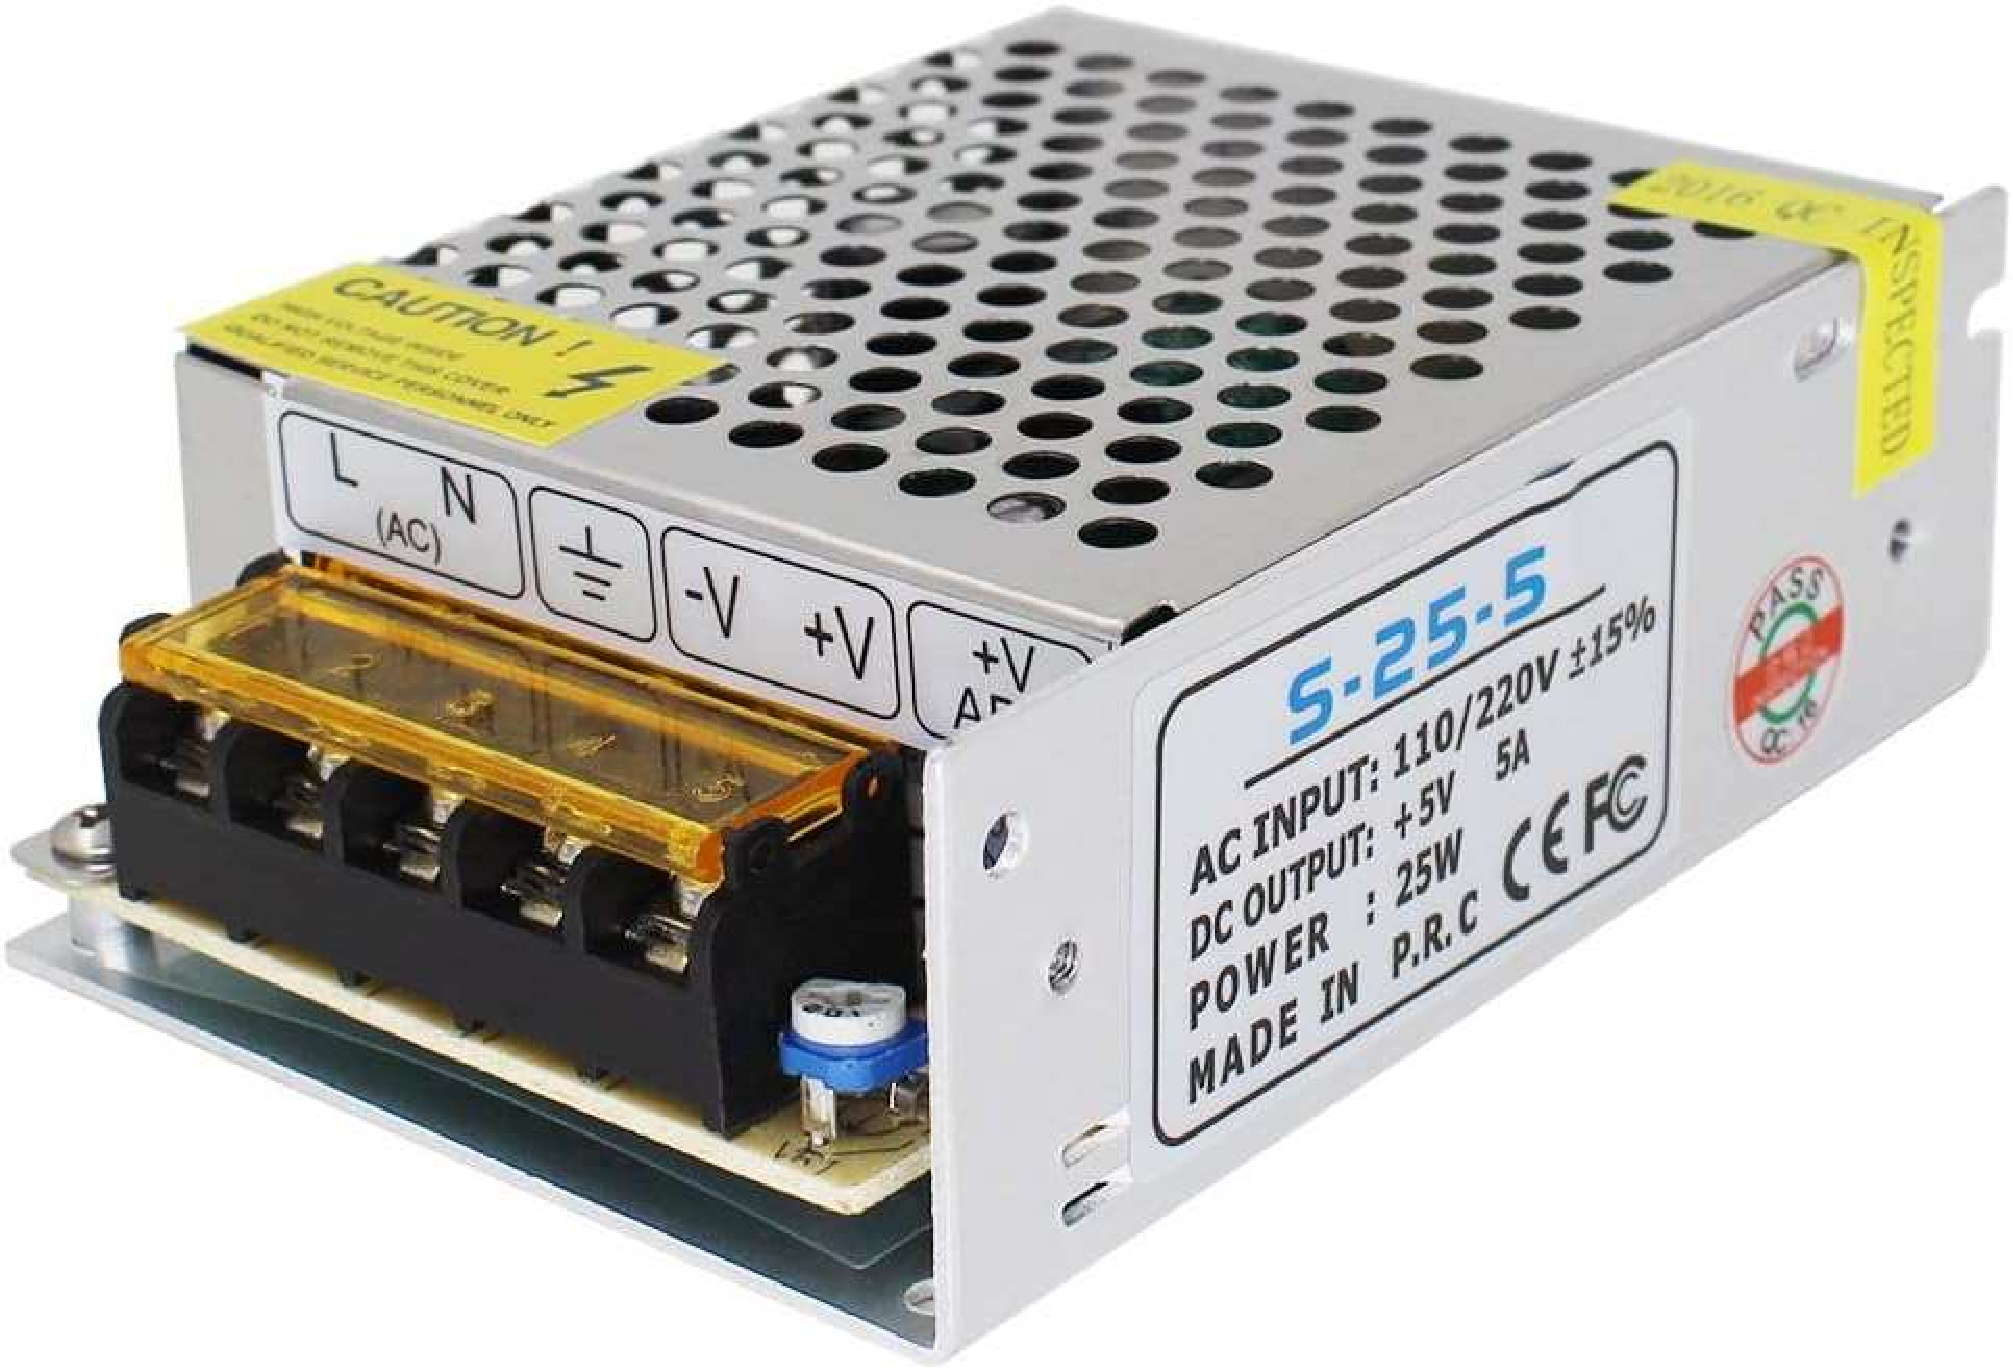
\includegraphics[width=0.45\textwidth]{Capitulos/3_hardware_softwares/3_figuras/f1_fonte.pdf}}
	\caption*{Fonte: elaborado pelo autor (2023).}
	\label{fig3:image_06}
\end{figure}



\subsubsection{Módulo Driver L298n}
\label{driver_l298n}

Para regular a velocidade no eixo do Motor CC série, empregou-se um Módulo Driver L298n, o qual possibilita controlar a injeção de potência entregue ao motor mediante a aplicação de um sinal PWM em sua entrada. Dessa forma, ao ajustar o sinal PWM, é possível obter uma tensão controlada aplicada de maneira precisa aos terminais do motor. A Figura \ref{fig3:image_07} ilustra o componente em questão.

\begin{figure}[!h]
	\centering
	\caption{Módulo Driver L298n.}
	\efbox{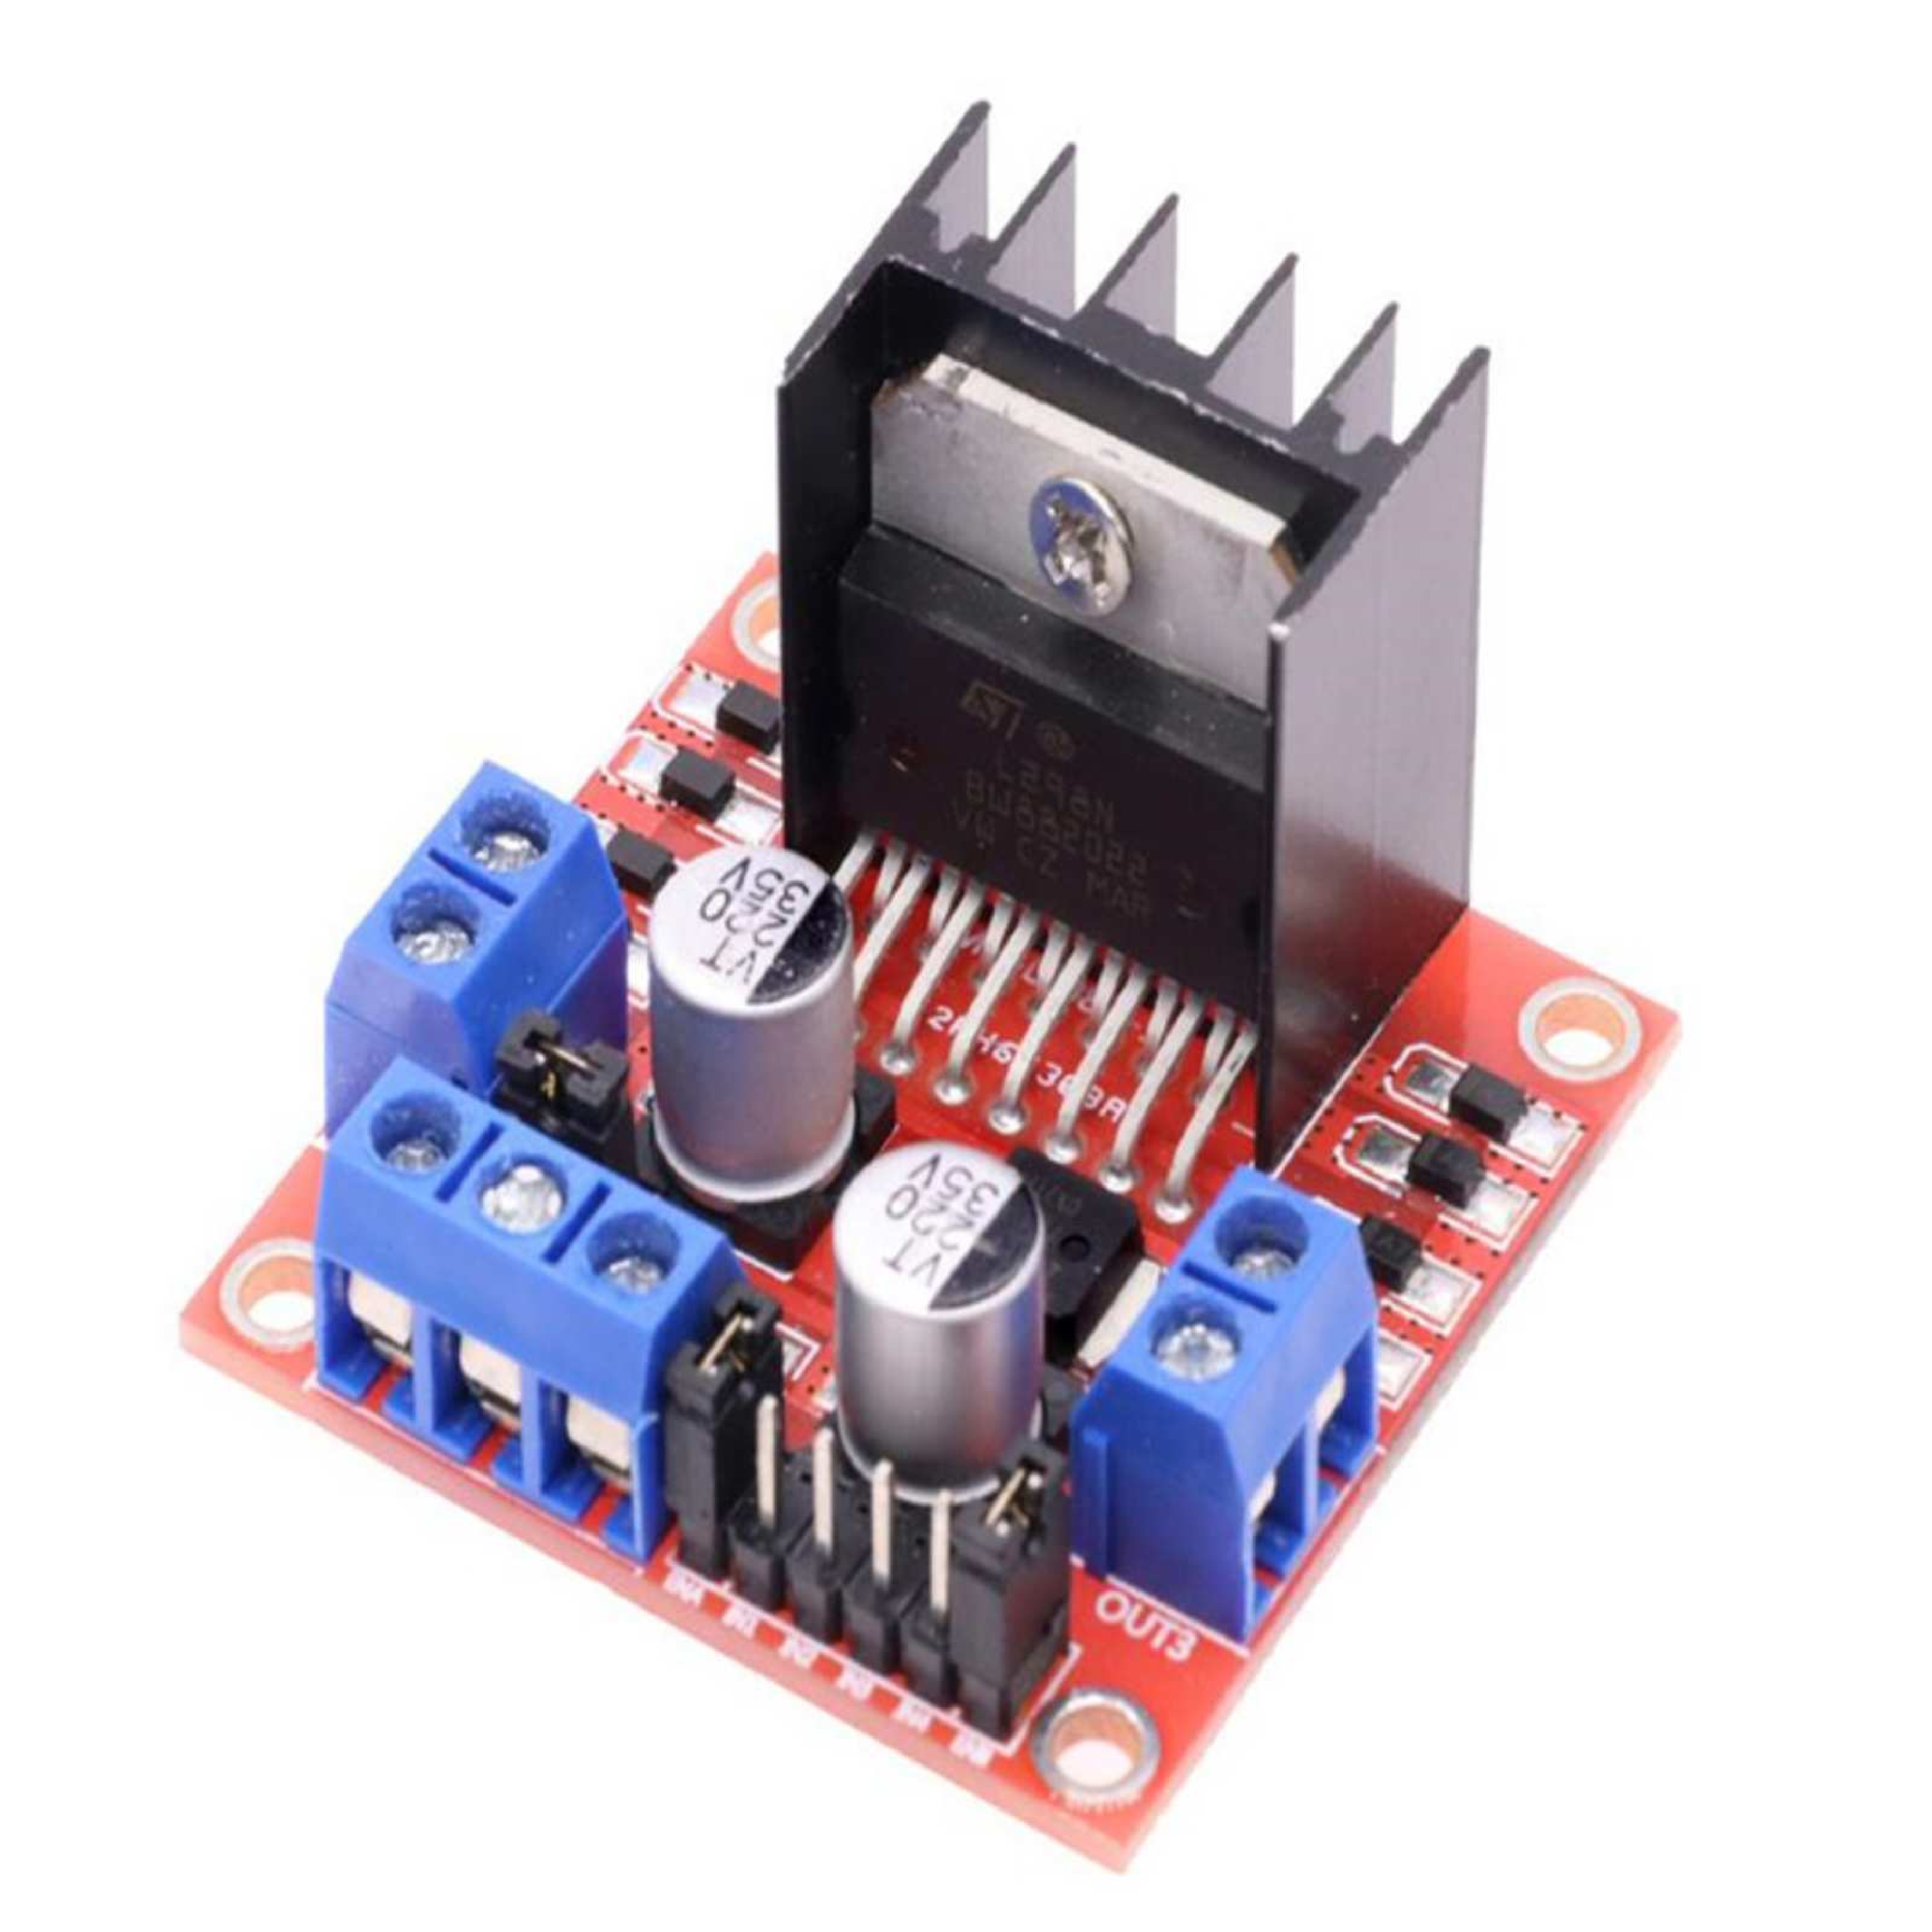
\includegraphics[width=0.45\textwidth]{Capitulos/3_hardware_softwares/3_figuras/f4_ponteH.pdf}}
	\caption*{Fonte: elaborado pelo autor (2023).}
	\label{fig3:image_07}
\end{figure}


\subsubsection{Conjunto (suporte motor cw/ccw hélice) para drones fpv racing quadcopter}


A obtenção da força de empuxo na extremidade do braço do Aeropêndulo foi realizada por meio de um conjunto composto por suporte, motor e hélice projetado originalmente para drones FPV Racing Quadcopter. Esse conjunto demonstrou ser ideal para aplicação no Aeropêndulo devido à sua eficiência e desempenho em ambientes dinâmicos. A Figura \ref{fig3:image_08} fornece uma representação visual esclarecedora desse componente crucial, destacando sua integração perfeita no contexto do experimento.


\begin{figure}[!h]
	\centering
	\caption{Conjunto (suporte motor cw/ccw hélice).}
	\efbox{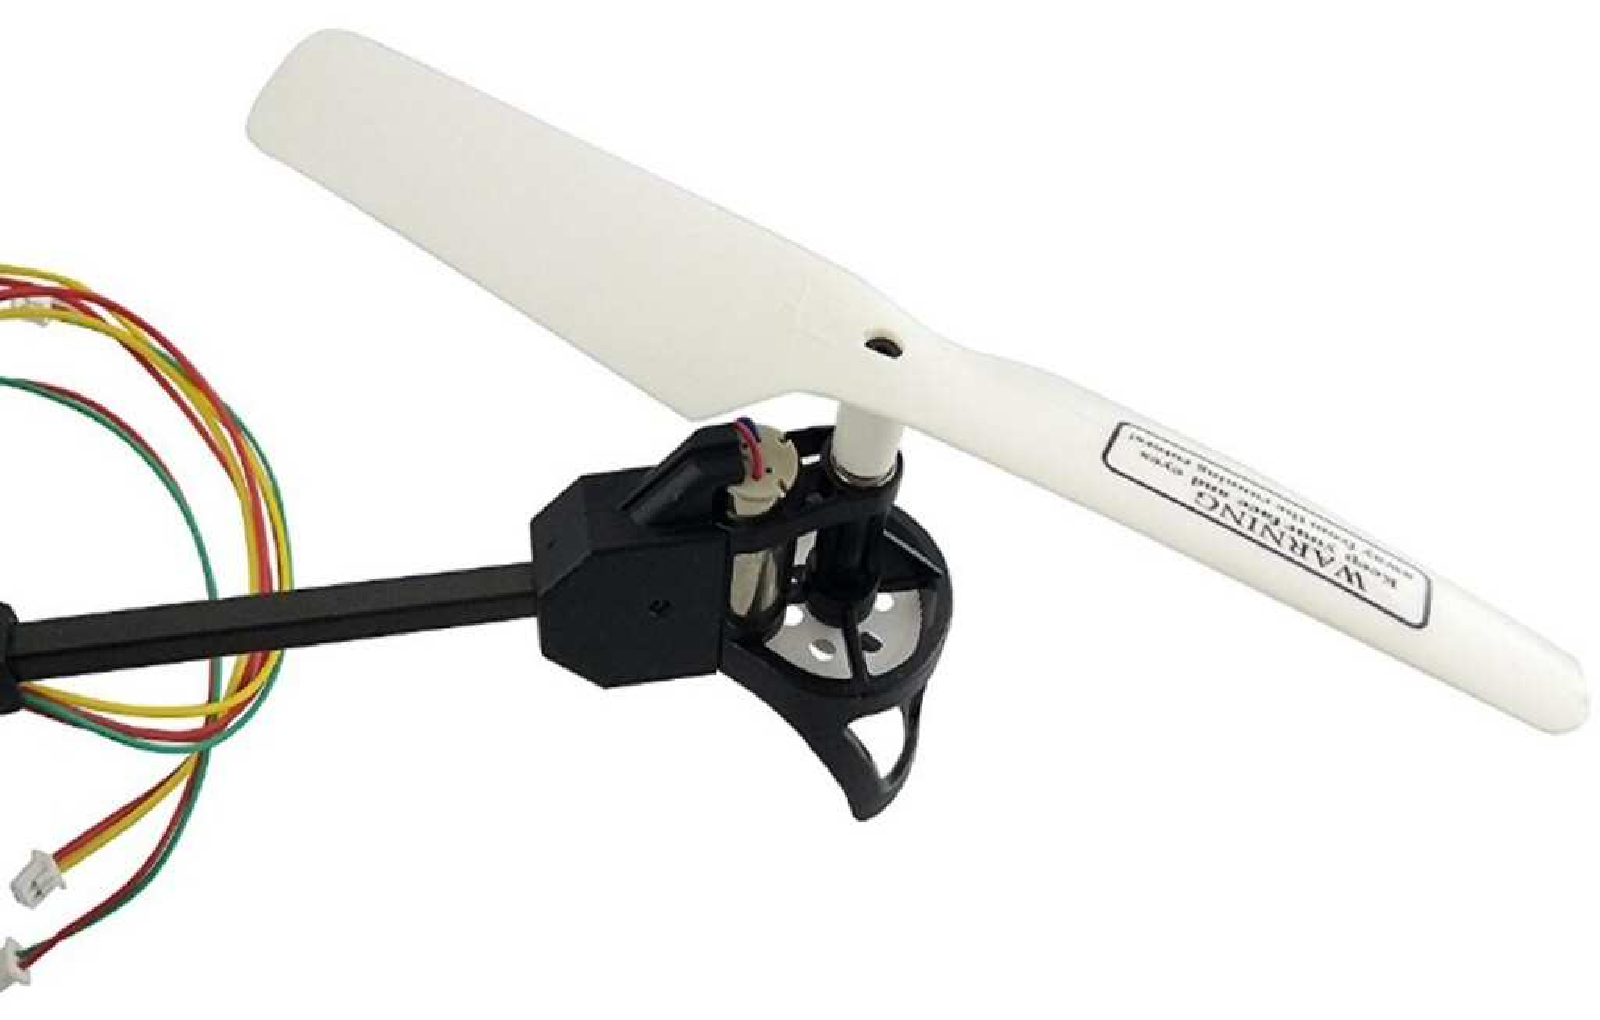
\includegraphics[width=0.5\textwidth]{Capitulos/3_hardware_softwares/3_figuras/f1_braco_aerop.pdf}}
	\caption*{Fonte: elaborado pelo autor (2023).}
	\label{fig3:image_08}
\end{figure}

\newpage
\subsubsection{Componentes eletrônicos (resistivos e capacitivos)}

Por fim, para que o sinal do sensor (Potenciômetro) seja de boa qualidade, foi usado um filtro RC série, dessa forma, empregou-se um capacitor de um resistor na implementar do filtro. A Figura \ref{fig3:image_09} corresponde aos componentes resistivos e a Figura \ref{fig3:image_10} aos componentes capacitivos.


\begin{figure}[!h]
         \centering
         \caption{Resistores.}
         \efbox{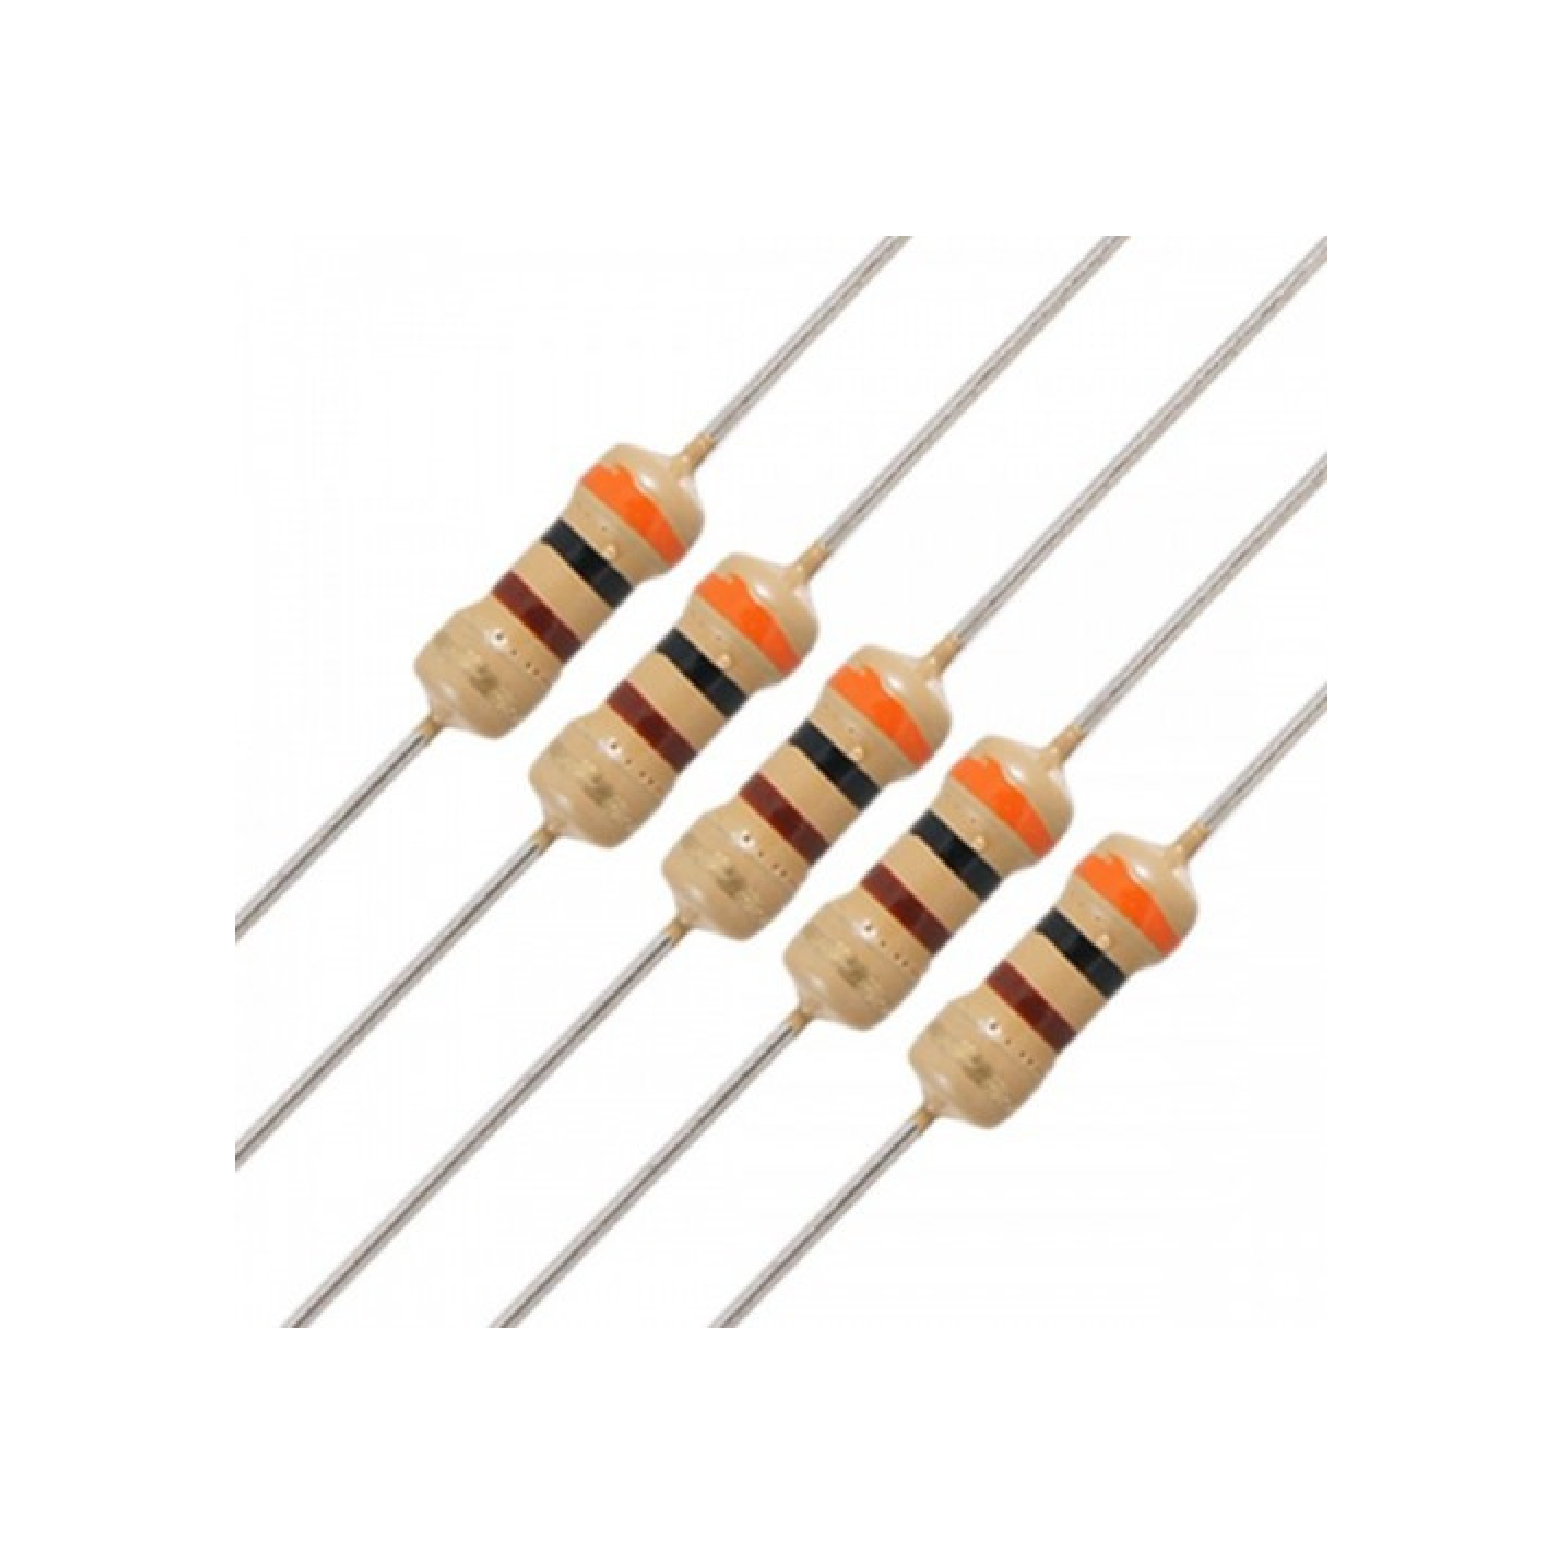
\includegraphics[width=0.5\textwidth, page=1]{Capitulos/3_hardware_softwares/3_figuras/res_cap.pdf}}
         \caption*{Fonte: elaborado pelo autor (2023).}
         \label{fig3:image_09}
\end{figure}

\begin{figure}[!h]
         \centering
         \caption{Capacitores.}
         \efbox{\includegraphics[width=0.5\textwidth, page=2]{Capitulos/3_hardware_softwares/3_figuras/res_cap.pdf}}
         \caption*{Fonte: elaborado pelo autor (2023).}
         \label{fig3:image_10}
\end{figure}


\subsection{Montagem do Protótipo}

\subsubsection{Parte Física}

O protótipo foi concebido visando a desmontagem da estrutura, permitindo um transporte mais conveniente. A construção física compreende três componentes com pontos de conexão estratégicos. Ademais, o braço do Aeropêndulo pode ser facilmente desacoplado no ponto de pivô, onde se conecta ao eixo do potenciômetro.

Para montar a estrutura, basta acoplar suas partes. Com isso, a componente estrutural estará pronta para uso. O resultado final do sistema ficou notavelmente estável, com a estrutura demonstrando rigidez suficiente para evitar vibrações indesejadas no braço do Aeropêndulo durante o acionamento.

\subsubsection{Parte Elétrica}


A Figura \ref{fig3:image_11} ilustra a dinâmica do fluxo de interligação do sistema elétrico do Aeropêndulo. Notavelmente, o microcontrolador desempenha um papel central ao gerar o sinal de controle PWM, realiza a leitura do sinal filtrado proveniente do sensor (Potenciômetro) e estabelecer comunicação com o computador através da interface serial. Adicionalmente, o driver é alimentado por uma fonte de tensão contínua de 5V, o qual amplifica e aplica o sinal de controle ao motor CC Série. Esta ação, por sua vez, resulta em uma variação angular no braço do Aeropêndulo por conta do empuxo gerado pelas hélices, impactando diretamente o estado do sensor (Potenciômetro) e sua saída correspondente.

\begin{figure}[!h]
	\centering
	\caption{Diagrama de comunicação do Aeropêndulo.}
	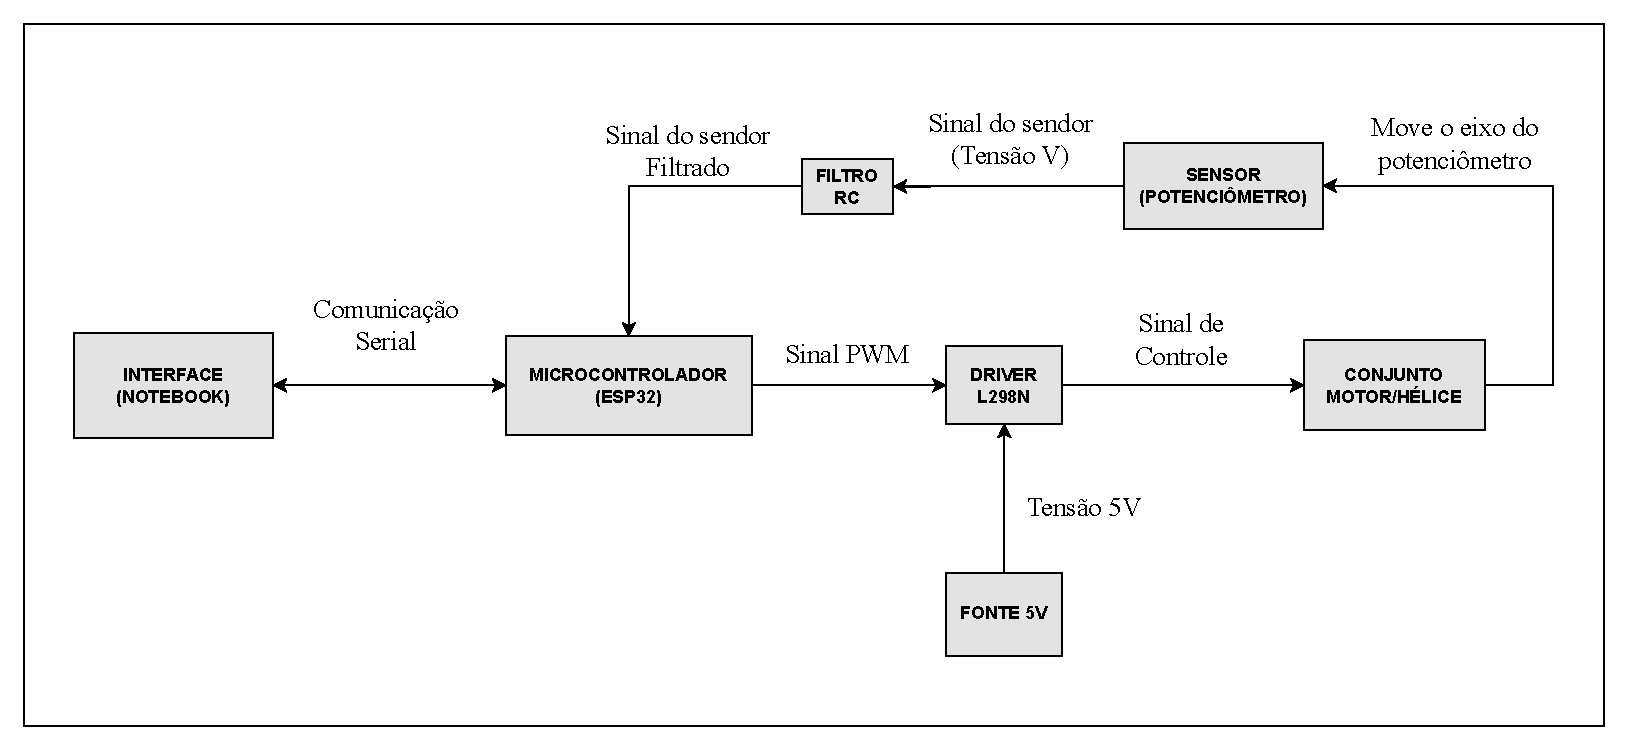
\includegraphics[width=0.9\textwidth, page=1]{Capitulos/3_hardware_softwares/3_figuras/diag_aerop.pdf}
	\caption*{Fonte: elaborado pelo autor (2023).}
	\label{fig3:image_11}
\end{figure}



O esquema de ligação dos componentes do sistema elétrico é exemplificado na Figura \ref{fig3:image_12}.

\begin{figure}[!h]
	\centering
    	\caption{Esquema de conexões elétricas do Aeropêndulo.}
	\efbox{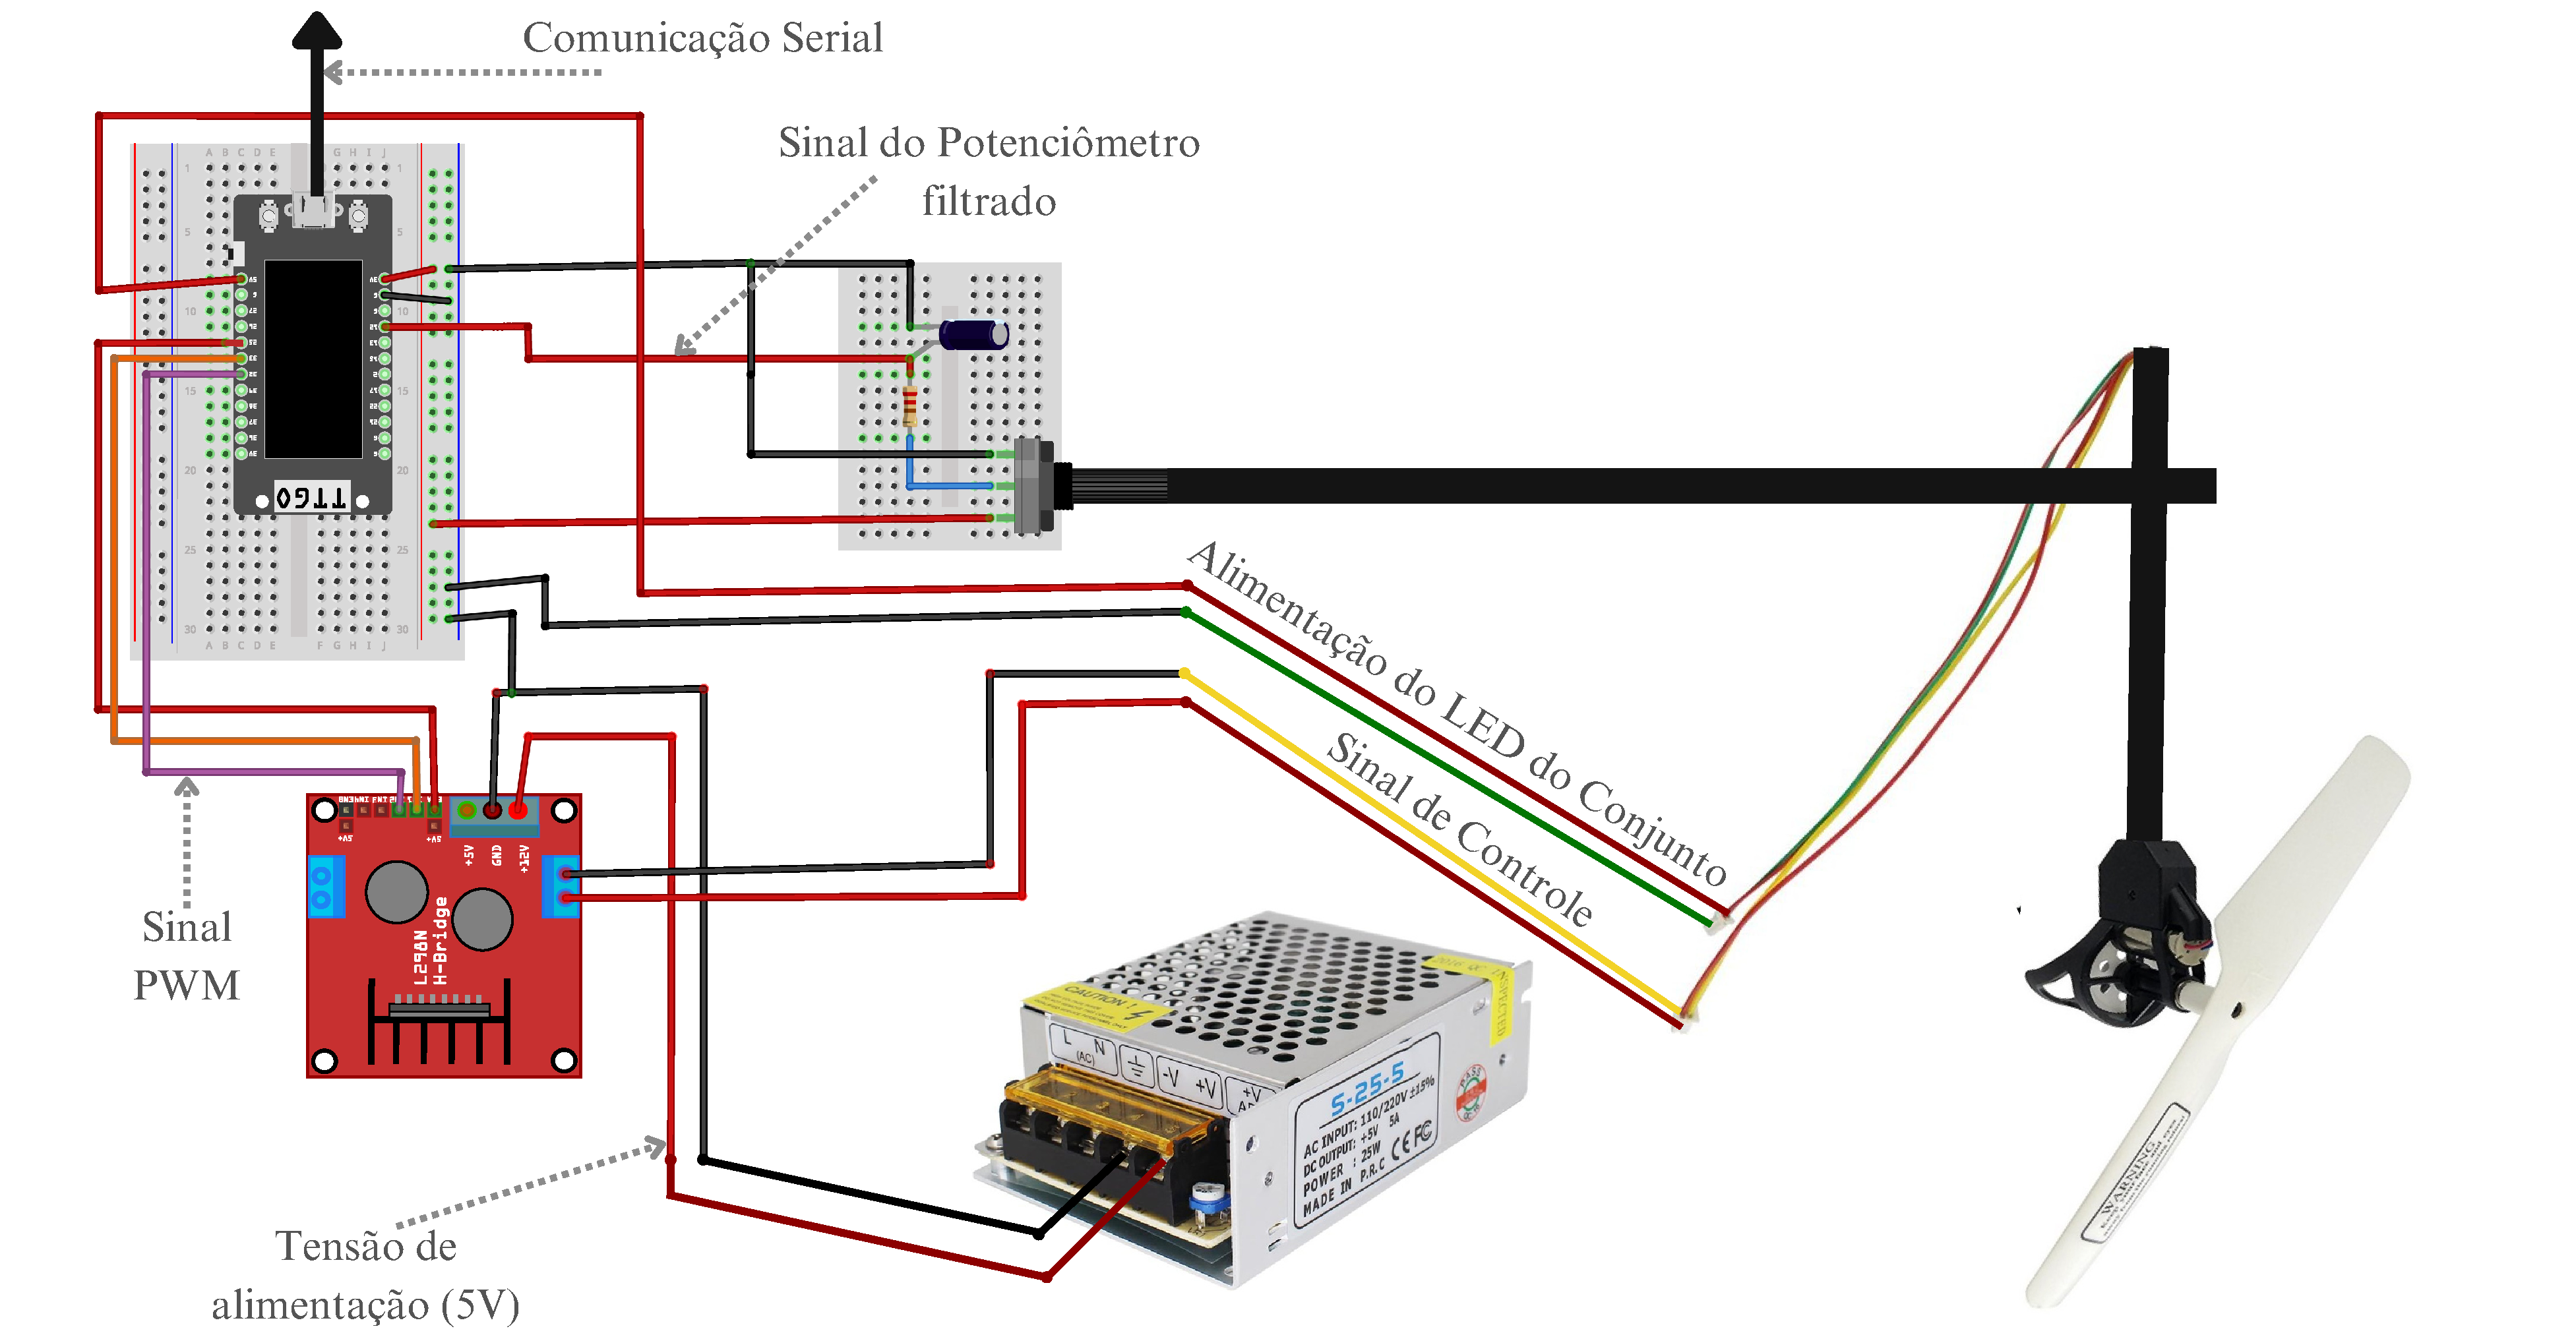
\includegraphics[width=1\textwidth, page=1]{Capitulos/3_hardware_softwares/3_figuras/esquema_eletrico_aerop.pdf}}
	\caption*{Fonte: elaborado pelo autor (2023).}
	\label{fig3:image_12}
\end{figure}

\vspace{2cm}


\section{Desenvolvimento dos Softwares}
\label{dev_softwares}
Para permitir a interação com o protótipo um conjunto de software foi desenvolvido, permitindo aos usuários aplicar diferentes conceitos de sistema de controle e obter uma visualização em tempo real dos estados do sistema através desses softwares, sendo eles, o firmware do microcontrolador, simulador 3D que usa o conceito de Gêmeo Digital, uma interface gráfica com um conjunto de funcionalidades capaz de manipular o sinal de referência e plotar os gráficos dos estados do sistema.

\subsection{Linguagens Python, C e C++}
Para o desenvolvimento dos softwares destinados à visualização de dados e ao simulador, a linguagem de programação escolhida foi o Python. Essa seleção se deu devido à natureza versátil da linguagem, que permite um desenvolvimento ágil de softwares para uma ampla gama de finalidades. Em paralelo, para a programação do microcontrolador, optou-se pelo uso das linguagens C/C++. Essa escolha se fundamenta na ampla adoção dessas linguagens na programação de sistemas embarcados, garantindo um ambiente propício para a eficaz implementação no microcontrolador.

A linguagem Python é amplamente reconhecida como uma linguagem de programação de alta qualidade, interpretada e de propósito geral. Ela desfruta de uma imensa popularidade em todo o mundo e é empregada em diversas aplicações, abrangendo campos como computação científica, ciência de dados, engenharia de software e inteligência artificial. Python se destaca por ser uma linguagem de programação de fácil aprendizado e utilização, mesmo para indivíduos com pouca experiência em codificação. Sua sintaxe clara e concisa contribui para a legibilidade e manutenibilidade do código.

Por essas razões, Python emerge como a escolha ideal para conduzir trabalhos de pesquisa e desenvolvimento. É uma ferramenta incrivelmente versátil e poderosa, capaz de lidar com uma extensa variedade de tarefas, desde a análise de dados até a criação de aplicações complexas.


Já C e C++ são linguagens de programação que se concentram na eficiência e na portabilidade. Elas são amplamente utilizadas no desenvolvimento de sistemas operacionais, drivers de dispositivos, compiladores e outros softwares críticos. C foi criada em 1972 por Dennis Ritchie para o desenvolvimento do sistema operacional Unix. C++ foi criada em 1983 por Bjarne Stroustrup como uma extensão de C para adicionar suporte à programação orientada a objetos.

C e C++ são linguagens de programação poderosas e flexíveis, mas também podem ser complexas e difíceis de aprender. Elas são recomendadas para desenvolvedores que precisam de um alto nível de controle sobre o desempenho e a portabilidade de seu código.


\subsection{ Gêmeo Digital}
Nesta seção, será elaborado o Gêmeo Digital do Aeropêndulo. O Gêmeo Digital representa um sistema gráfico computacional que reproduz em tempo real a dinâmica do protótipo. Isso permite a virtualização do Aeropêndulo, possibilitando a observação da mesma dinâmica do sistema físico, agora em um ambiente gráfico computacional 3D. Essa virtualização é viabilizada pela obtenção do estado atual do braço do Aeropêndulo por meio de comunicação serial.

Para o desenvolvimento do Gêmeo Digital, utilizou-se a biblioteca VPython, essa biblioteca possui um conjunto de funções que permite criar objetos 3D capazes de realizar movimentos rotacionais de translacionais, além disso, é possível plotar gráficos em tempo real. A figura \ref{fig3:image_13_1} ilustra a interface do simulador já finalizado, pode-se observar que a interface é composta de duas partes principais, uma que implementa o ambiente 3D com o Aeropêndulo e a outra gera os gráficos do sinal de referência e de saída.

Com a finalidade de atualizar os estados dos gráficos e a posição angular do gêmeo digital em tempo real a aplicação se comunica com a interface gráfica, subseção \ref{interface_graica}, com isso é possível realizar a atualização dos estados do gráfico assim como do gêmeo digital tendo como entrada os sinais dos estados do protótipo.

\begin{figure}[!h]
	\centering
	\caption{Gêmeo Digital - Simulador com VPython.}
	\efbox{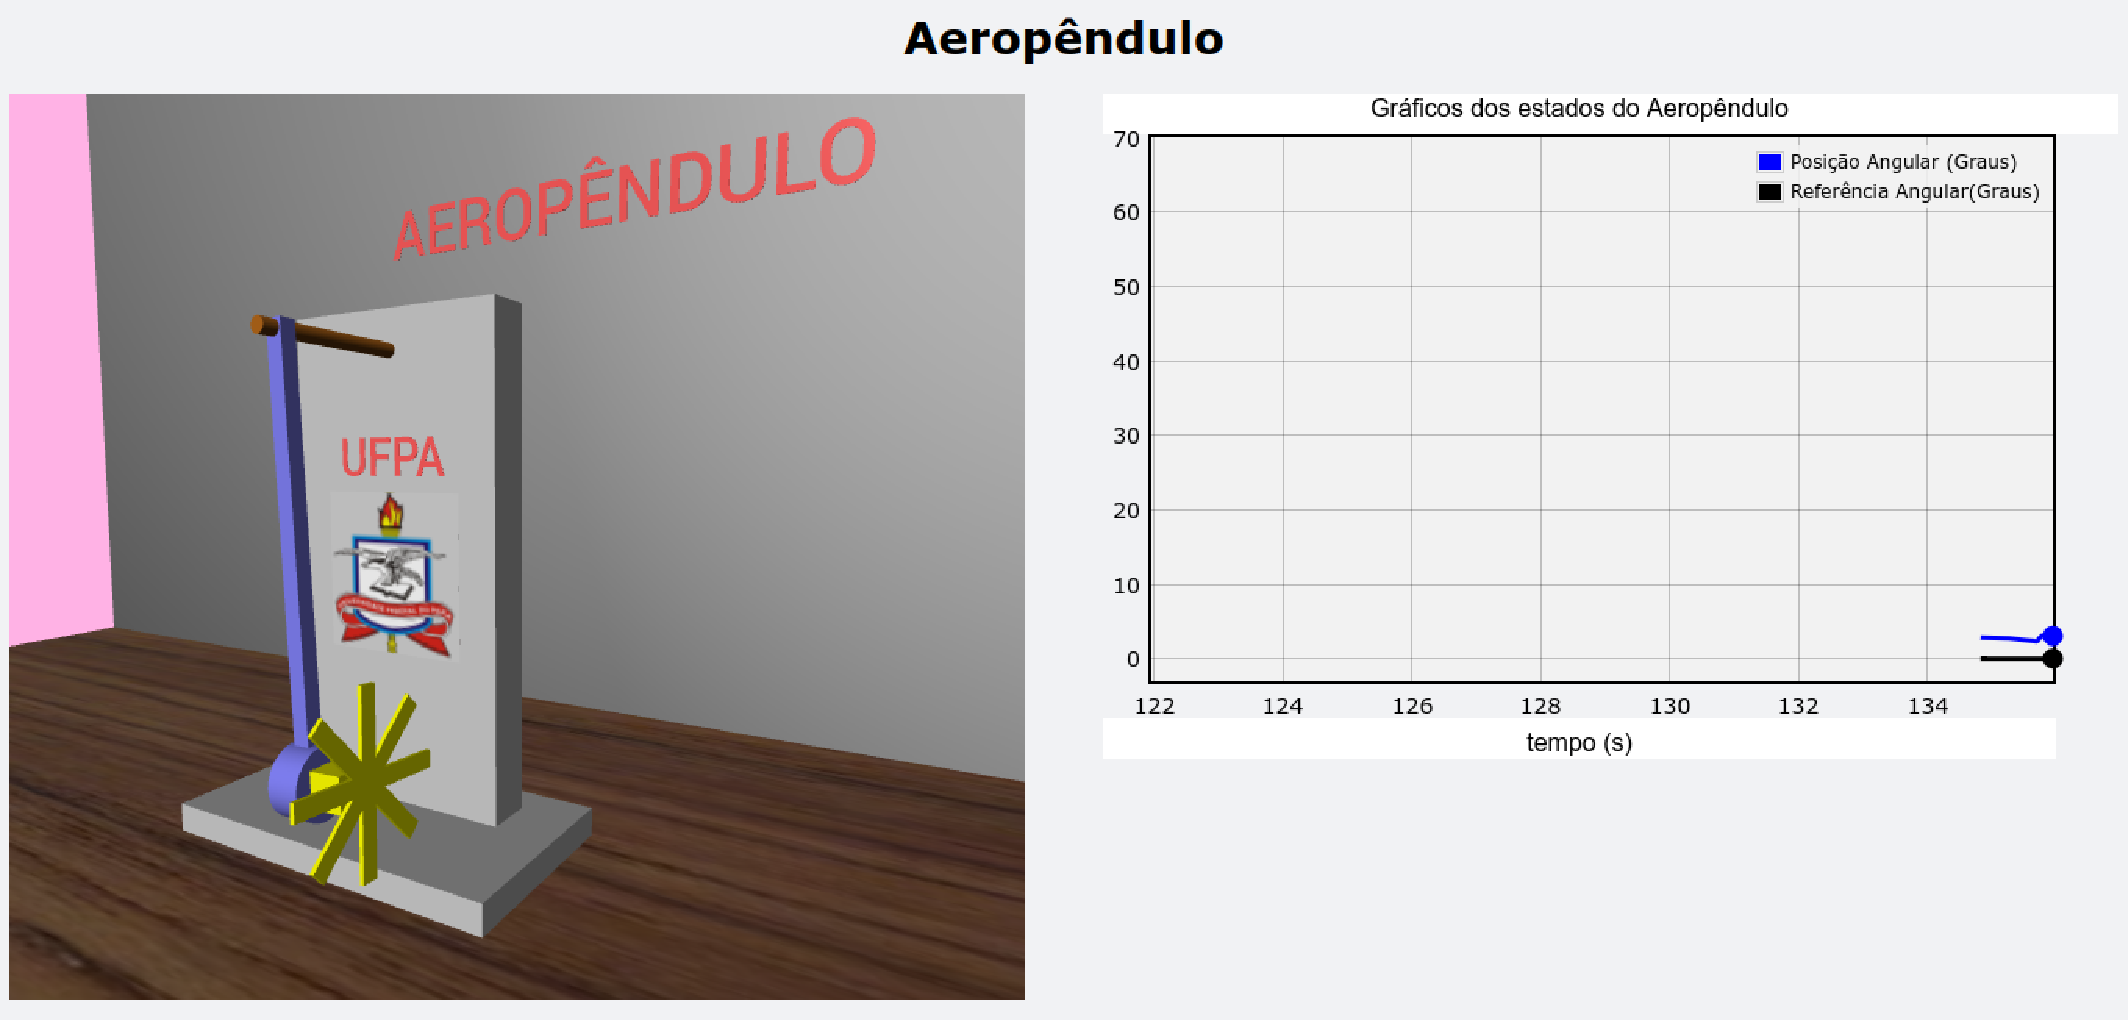
\includegraphics[width=1\textwidth]{Capitulos/3_hardware_softwares/3_figuras/simulador.pdf}}
        \vspace{0.001cm}
	\caption*{Fonte: elaborado pelo autor (2023).}
	\label{fig3:image_13_1}
\end{figure}

% O gêmeo digital do aeropêndulo foi derivado de um projeto que o Autor desse TCC participou, intitulado \textbf{Laboratório Virtual para Sistemas Dinâmicos e Controle na Faculdade de Engenharia Elétrica da UFPA-Tucuruí}, a partir desse projeto foi ...

\newpage
\subsubsection{Biblioteca VPython}

Conforme o site oficial \cite{vpython}, O VPython, por ser desenvolvido com a linguagem Python, é uma ferramenta versátil para a criação de animações 3D navegáveis. Ele é fácil de aprender e usar, mesmo para pessoas com pouca experiência em programação. No entanto, ele também oferece uma ampla gama de recursos para programadores e pesquisadores experientes.

Ao criar uma simulação com VPython e executá-la, o simulador será renderizado no navegador de internet padrão do sistema operacional.


\subsubsection{Arquitetura do Gêmeo Digital}

Para implementar o simulador a arquitetura do sistema consiste de um módulo para gerar os gráficos de linha e outro para desenhar o simulador 3D, existe um módulo que integra e atualiza os estados dos gráficos de linha e do simulador 3D, a figura \ref{fig3:image_13} mostra como a estrutura do simulador foi pensada, o último bloco é a interface gráfica, subseção \ref{interface_graica}, responsável por obter os estados do sistema real, com isso, é possível usar a velocidade angular real do protótipo como entrada para o gêmeo digital, isso faz com que a dinâmica do protótipo seja reproduzida no gêmeo digital, além disse, é possível obter os sinais de referência e de saída e atualizar os gráfios que compõem a interface do simulador.

\begin{figure}[!h]
	\centering
	\caption{Diagrama da arquitetura do Gêmeo Digital.}
	\efbox{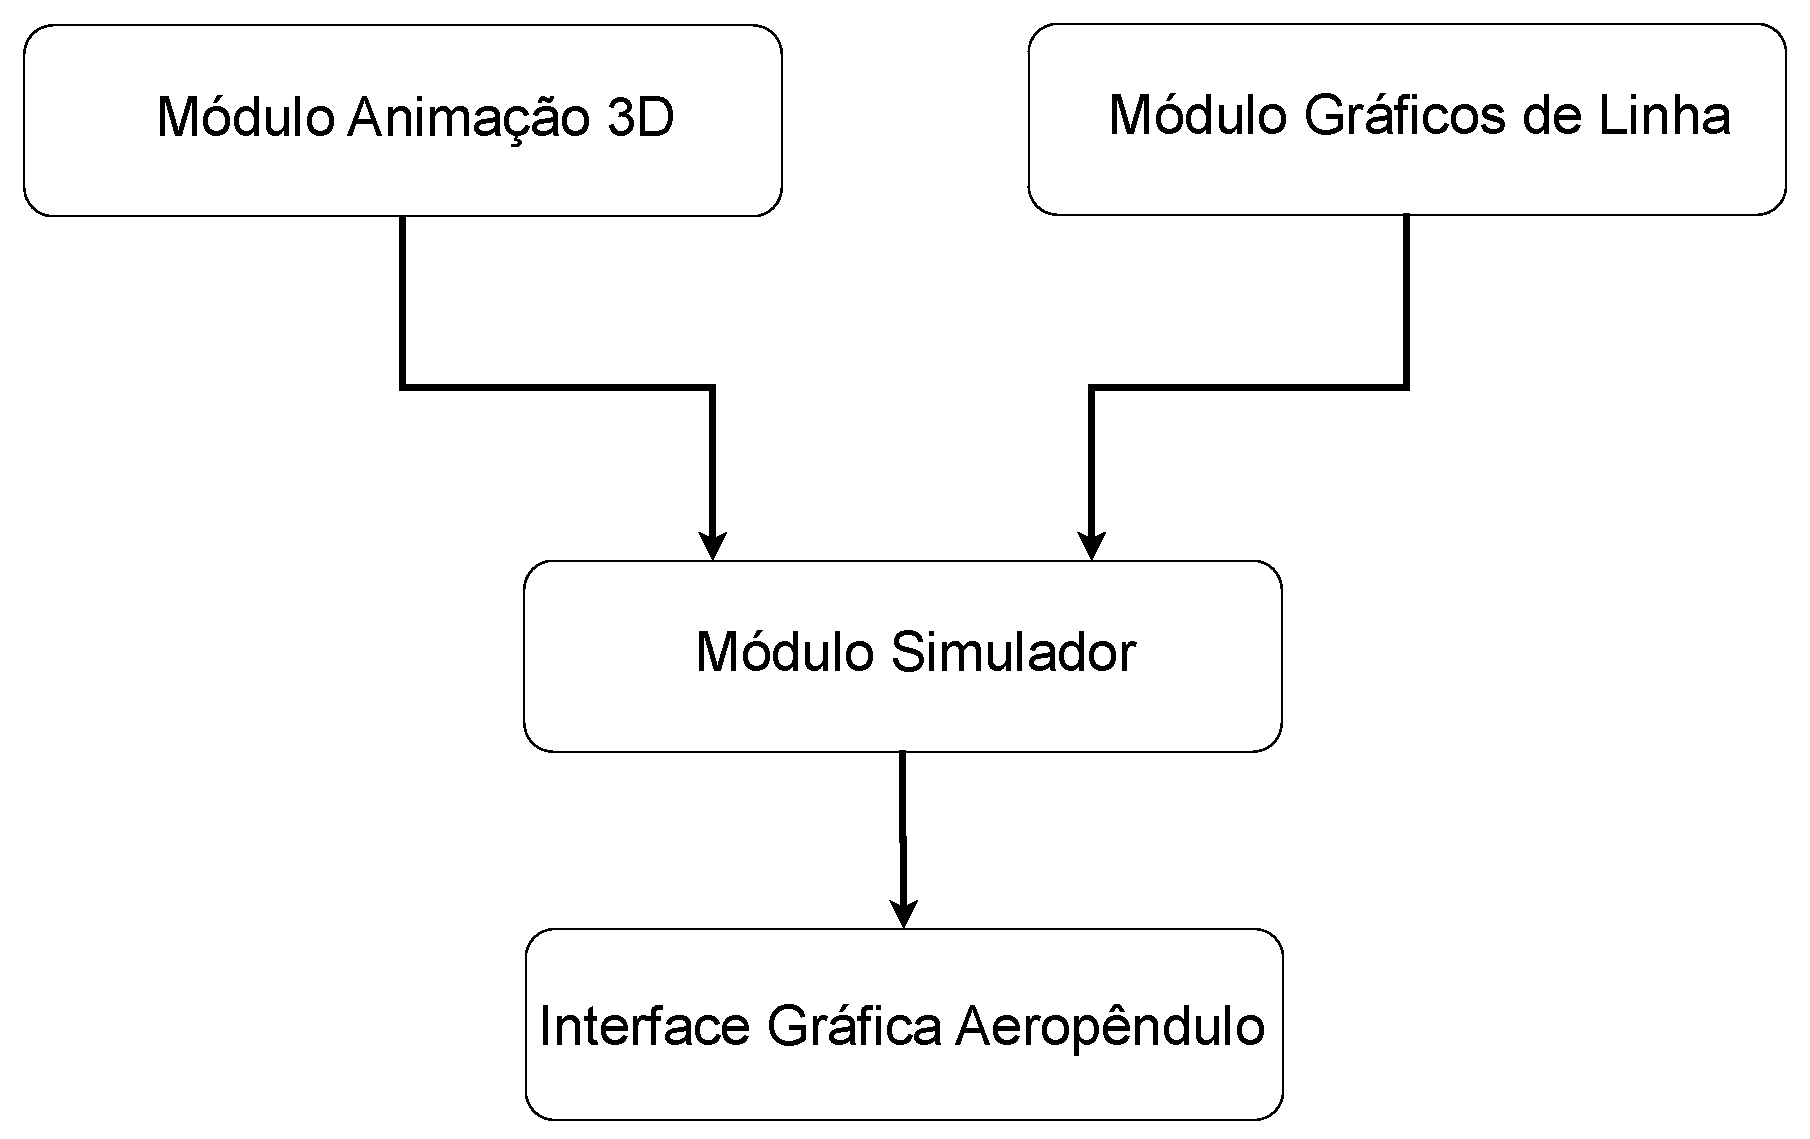
\includegraphics[width=0.55\textwidth, page=1]{Capitulos/3_hardware_softwares/3_figuras/arquitetura_simulador.pdf}}
        \vspace{0.2cm}
	\caption*{Fonte: elaborado pelo autor (2023).}
	\label{fig3:image_13}
\end{figure}


\newpage

O \textbf{Módulo Simulador}, código abaixo, recebe como parâmetro  o \textbf{Módulo Animação 3D} e o \textbf{Módulo Gráficos de Linha}, a partir disso  é implementada uma Classe Python usando a ideia de programação orientada a objetos para realizar a construção tanto da parte gráfica quanto do simulador 2D.

\vspace{0.5cm}

\begin{lstlisting}[language=python, numbers=left, label=python-example, captionpos=b, caption={Classe que implementa o Gêmeo Digital}]
import vpython as vp

# Modulos do Gemeo Digital desenvolvidos
from .interfaces.graficos_aeropendulo import GraficosInterface
from .interfaces.animacao_aeropendulo import AnimacaoAeropenduloInterface
from .interfaces.simulador import SimuladorInterface


class Simulador(SimuladorInterface):
    def __init__(
            self, graficos: GraficosInterface,
            animacao_aeropendulo: AnimacaoAeropenduloInterface) -> None:
        self.t = 0
        self.t_ant = 0
        self.ts = 0
        self.theta_rad = 0
        self.theta_rad_ant = 0
        self.dtheta_rad = 0
        # Instanciando um objeto AeropenduloAaeropendulo()
        self.animacao_aeropendulo = animacao_aeropendulo

        # Instanciando um objeto para plotagem dos graficos
        # dinamicos dos estados do Aeropendulo
        self.g = graficos
        self.graf, self.plot1, self.plot2 = self.g.graficos()  # noqa

    def grau2rad(self, graus):
        return (graus)*(vp.pi/180.0)

    def rotate(self, angle) -> None:
        self.valor_angle = self.grau2rad(angle)
        self.animacao_aeropendulo.aeropendulo.rotate(
            axis=vp.vec(0, 0, 1),
            angle=self.valor_angle,
            origin=vp.vec(0, 5.2, 0))
        self.animacao_aeropendulo.set_posicao_helice(self.valor_angle)

    def atualizar_estados(self, t, theta, ref):
        self.t = t
        self.ts = self.t - self.t_ant
        self.theta_rad = self.grau2rad(theta)
        try:
            self.dtheta_rad = (
                self.theta_rad - self.theta_rad_ant
                )/self.ts
        except Exception as exception:
            print(exception)

        # Atualiza o angulo do Aeropendulo
        self.animacao_aeropendulo.aeropendulo.rotate(
                        axis=vp.vec(0, 0, 1),
                        angle=self.dtheta_rad*self.ts,
                        origin=vp.vec(0, 5.2, 0))

        # Animacao da dinamica da Helice
        self.animacao_aeropendulo.update_helice(self.dtheta_rad, self.ts)

        # print(x[1] + interface.valor_angle)
        # Grafico do angulo.
        self.plot1.plot(t, theta)
        # Grafico do sinal de referencia
        self.plot2.plot(t, ref)

        self.t_ant = t
        self.theta_rad_ant = self.theta_rad

\end{lstlisting}

Para atualizar a dinâmica do braço do Aeropêndulo do Gêmeo Digital, a classe \textbf{Simulador} é importada no outro software, seção \ref{interface_graica} que implementa a comunicação com o protótipo e obtêm os estados do sistema real, assim é possível atualizar o Gêmeo Digital com dados reais do braço do Aeropêndulo.

Logo, o código desenvolvido para implementar o Gêmeo Digital deve ser importado no código que implementa a Interface Gráfica de Usuário, seção \ref{interface_graica}.
%
\subsection{Interface Gráfica para Configuração, visualização e aquisição de dados da Planta}
\label{interface_graica}

A interface gráfica consiste de um menu com diferentes opções de controle e visualização dos sinais do sistema e um conjunto de gráficos dinâmicos para visualizar os estados do sistema em tempo real. A figura \ref{fig3:image_14} mostra a interface do sistema. No entanto, além da parte visual existe a parte de aquisição e processamento de dados, em TI essa parte e chamada de Back-end, o projeto possui uma classe para realizar essa parte de aquisição e tratamento de dados, além de uma classe para detectar automaticamente o microcontrolador conectado a porta USB.

Para ser possível realizar os ensaios, modificação de parâmetros do sinal de referência e coletas de dados é preciso que o microcontrolador execute o firmware, subseção \ref{firmware}, desenvolvido especificamente para esse propósito, dessa forma, a interface gráfica, figura \ref{fig3:image_14}, conseguirá realizar o pre-processamentos dos dados e plotar os sinais nos gráficos e demais atualizações nos softwares.

\begin{figure}[!h]
	\centering
	\caption{Interface Gráfica.}
	\efbox{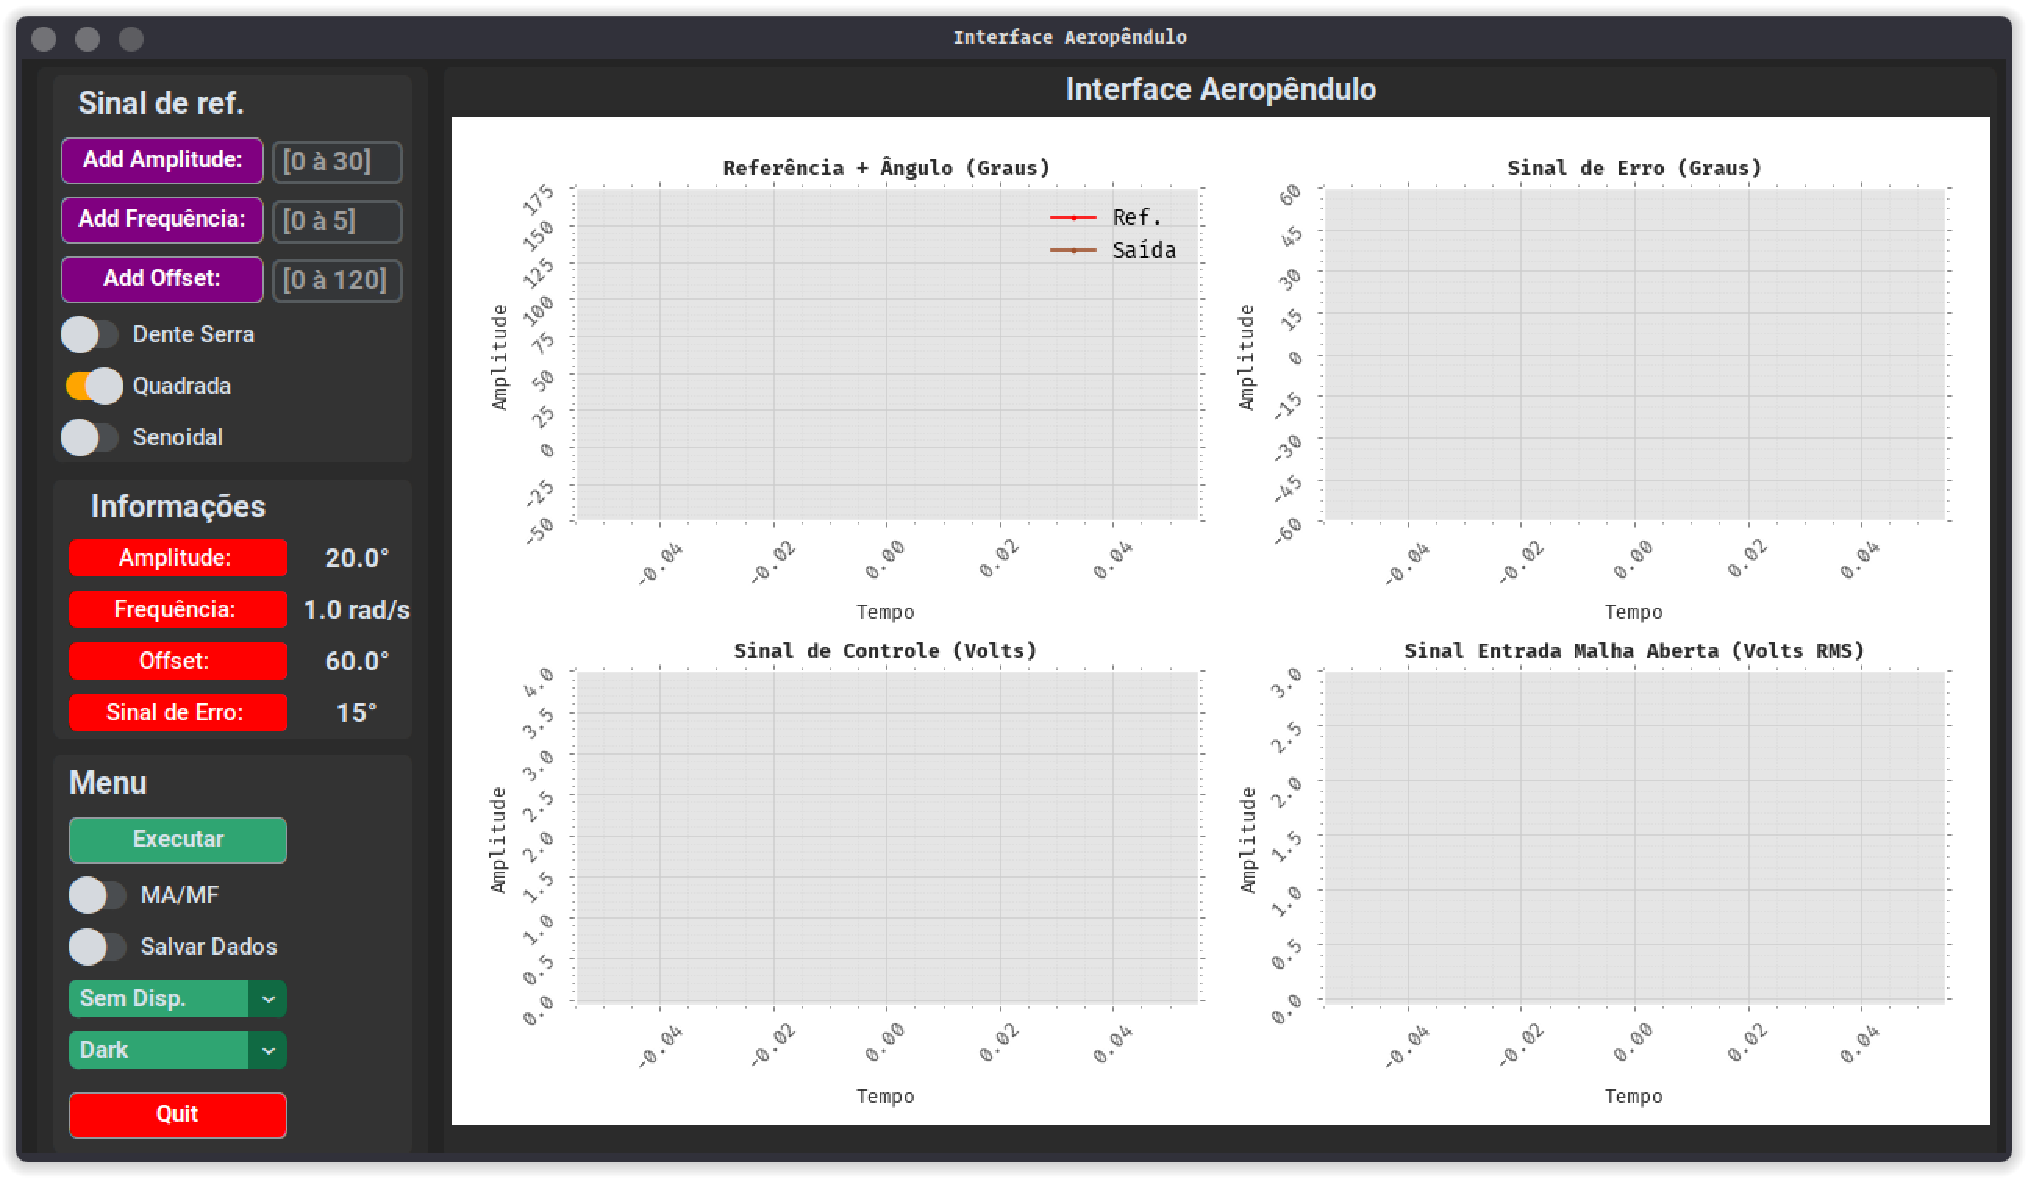
\includegraphics[width=0.9\textwidth]{Capitulos/3_hardware_softwares/3_figuras/interface.pdf}}
        \vspace{0.001cm}
	\caption*{Fonte: elaborado pelo autor (2023).}
	\label{fig3:image_14}
\end{figure}



O código a seguir realiza a importação de todos os módulos Python desenvolvidos tanto para a implementação da Interface Gráfica do Usuário quanto para o Gêmeo Digital. Com base nisso, foi elaborado um algoritmo que organiza adequadamente o funcionamento de ambos os softwares, viabilizando uma comunicação eficiente entre eles.

\vspace{0.5cm}

\begin{lstlisting}[language=python, numbers=left, label=py2, caption={Código que execulta a Interface Gráfica e o Gêmeo Digital.}]
import argparse
# Modulos da Interface Grafica de Usuario
from src_interface import InterfaceAeropendulo
from src_interface.graficos_sinais import GraficosSinais

# Modulos do Gemeo Digital
from simulador_aeropendulo.simulador import Simulador
from simulador_aeropendulo.graficos_aeropendulo import Graficos
from simulador_aeropendulo import AnimacaoAeropendulo

class RunInterface:
    def __init__(self) -> None:
        simular = self.get_args()
        self.runinterface(simular)

    def get_args(self) -> bool:
        parser = argparse.ArgumentParser()
        parser.add_argument(
            "-simular", "--Output",
            help="""Para habilitar o simulador, use a sintax:
                    python rungui.py -simular sim""")
        args = parser.parse_args()
        if args.Output == "sim":
            return True
        else:
            return False

    def runinterface(self, simular):
        if simular:
            simulador = Simulador(Graficos(), AnimacaoAeropendulo())
        else:
            simulador = None
        InterfaceAeropendulo(GraficosSinais,
                             simulador, baud_rate=115200,
                             amostras=80.0, tela_fixa=True)

if __name__ == "__main__":
    RunInterface()

\end{lstlisting}


Para roda a Interface Gráfica de Usuário juntamente com o Gêmeo Digital usa-se o seguinte comando no terminal estando dentro da pasta a partir do terminal:

\vspace{0.5cm}

\begin{lstlisting}[language=python]
python rungui.py -simular sim
\end{lstlisting}

Para roda apenas a Interface Gráfica de Usuário usa-se o seguinte comando no terminal:

\vspace{0.5cm}

\begin{lstlisting}[language=python]
python rungui.py
\end{lstlisting}



\subsubsection{Biblioteca CustomTkinter e Matplotlib}

Para o desenvolvimento da parte gráfica do software foi usado as bibliotecas CustomTkinter e Matplotlib, onde a biblioteca CustomTkinter implementa a estrutura de tela, botões, entradas de texto da aplicação e os módulos \textit{Matplotlib.pyplot} e \textit{Matplotlib.animation} possibilitam gerar gráficos em tempo real em conjunto com CustomTkinter.

Conforme \cite{customtkinter} explica no site oficial da biblioteca, "CustomTkinter é uma biblioteca de UI de desktop python baseada em Tkinter, que fornece widgets de aparência moderna e totalmente personalizáveis. Com CustomTkinter você terá uma aparência consistente em todas as plataformas de desktop (Windows, macOS, Linux)."

De acordo com \cite{matplotlib}, "Matplotlib é uma biblioteca abrangente para criar visualizações estáticas, animadas e interativas em Python. Matplotlib torna as coisas simples fáceis e as difíceis possíveis."

\subsubsection{Biblioteca PySerial, NumPy e Pandas}
Já para implementar o Back-end foram utilizadas as bibliotecas PySerial, NumPy e Pandas. Sendo que a biblioteca PySerial tem por finalidade realizar a comunicação entre o computador e o microcontrolador usando o protocolo seial via entrada USB, já o NumPy teve sua aplicação no processo de criação das matrizes contendo os dados lidos pela PySerial, por fim, para salvar os dados de ensaio foi usada a biblioteca Pandas, sendo salvos no formato CSV.

Conforme \cite{pyserial}, "A biblioteca PySerial possibilita a comunicação serial entre o computador e o microcontrolador usando conexão USB, Este módulo encapsula o acesso à porta serial. Ele fornece backends para Python rodando em Windows, OSX, Linux, BSD (possivelmente qualquer sistema compatível com POSIX) e IronPython. O módulo denominado “serial” seleciona automaticamente o backend apropriado."

% \citeonline[p.~11]{numpy_opl}   - Exemplo

De acordo com \cite{numpy_opl}, "O NumPy, uma biblioteca essencial para Python, oferece recursos robustos para realizar cálculos numéricos, sendo seu elemento central o ndarray, também conhecido como tensor. O ndarray se destaca por sua homogeneidade, exigindo que todos os elementos pertençam ao mesmo tipo, em contraste com as listas Python."

Segundo \cite{pandas}, site oficial da ferramenta, "pandas é uma ferramenta de análise e manipulação de dados de código aberto rápida, poderosa, flexível e fácil de usar, construído sobre a linguagem de programação Python."


\subsubsection{Descrição das partes da interface gráfica}

Nessa subseção será detalhado as partes do software, a figura \ref{fig3:image_15} está enumerando as partes e suas descrições estão logo abaixo.

\begin{figure}[!h]
	\centering
	\caption{Partes da Interface Gráfica.}
	\efbox{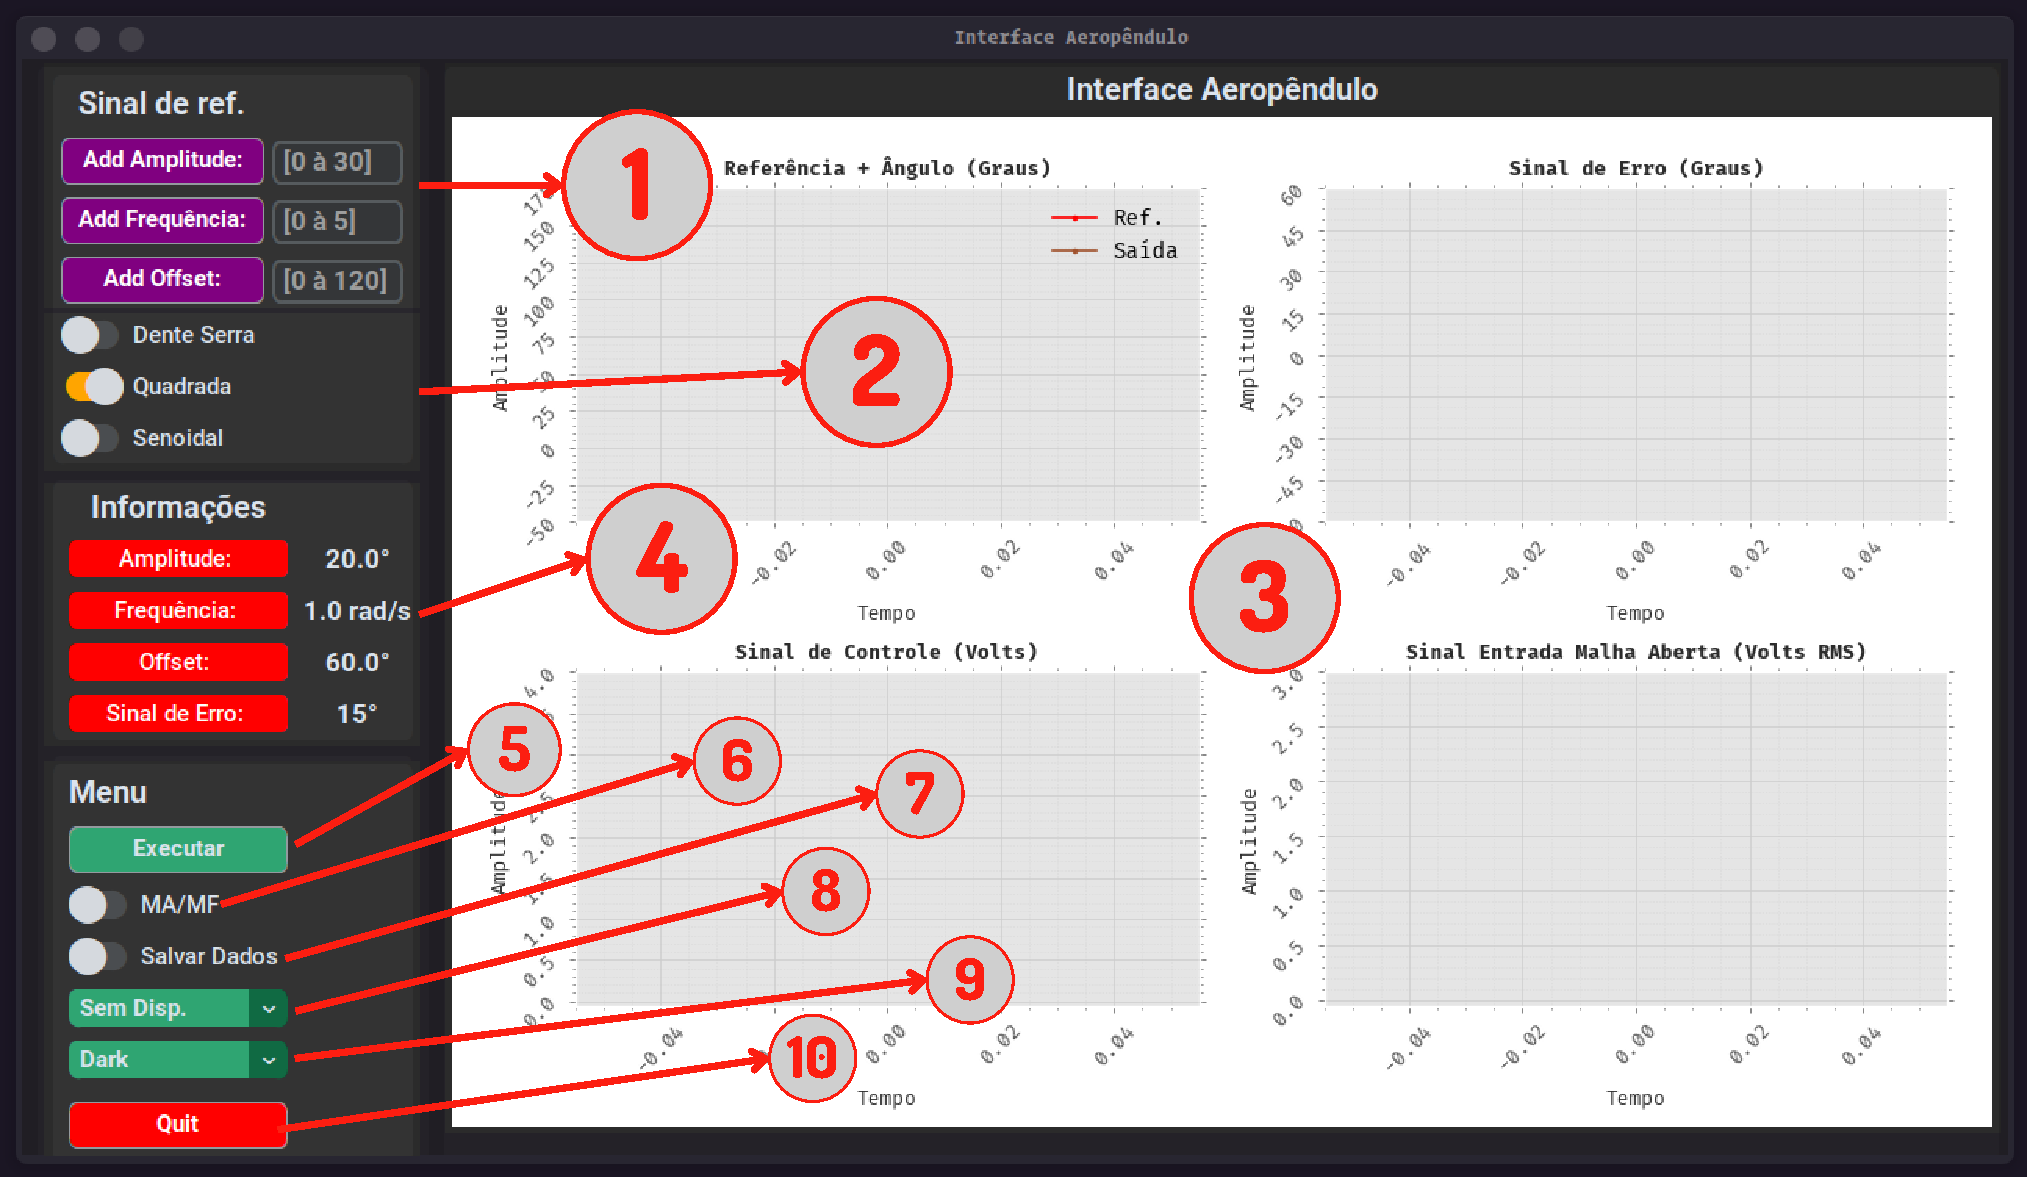
\includegraphics[width=0.95\textwidth]{Capitulos/3_hardware_softwares/3_figuras/interface_partes.pdf}}
	\caption*{Fonte: elaborado pelo autor (2023).}
	\label{fig3:image_15}
\end{figure}



\subsubsection*{\textit{Item 1: Sinal de Referência}}

Essa parte do software configura os sinais de referência aplicado ao sistema em malha fechada.


\begin{itemize}
        \setlength{\itemsep}{-2pt}
	\item  \textbf{Add Amplitude:} Configura a amplitude do sinal aplicado a entrada do sistema;
        \item  \textbf{Add Frequência:} Configura a frequência do sinal aplicado a entrada do sistema;
        \item  \textbf{Add Offset:} Configura a amplitude do offset, ponto de equilíbrio, aplicado a entrada do sistema.
\end{itemize}


\subsubsection*{\textit{Item 2: Seleção do Sinal de referência}}


\begin{itemize}
        \setlength{\itemsep}{-2pt}
	\item \textbf{Onda Serra:} Ao selecionar essa opção o sinal aplicado ao sistema será um dente de serra com as configurações de amplitude, frequência e offset conforme configurado nos três primeiros sub itens;
        \item \textbf{Quadrada:} Ao selecionar essa opção o sinal aplicado ao sistema será uma onda quadrada com as configurações de amplitude, frequência e offset conforme configurado nos três primeiros sub itens.;
        \item \textbf{Senoidal:} Ao selecionar essa opção o sinal aplicado ao sistema será uma onda senoidal com as configurações de amplitude, frequência e offset conforme configurado nos três primeiros sub itens.
\end{itemize}

\subsubsection*{\textit{Item 3: Gráficos}}

\begin{itemize}
        \setlength{\itemsep}{-2pt}
	\item \textbf{Gráficos:} Nesse item que são plotados os gráficos dos estados do sistema em tempo real.
\end{itemize}

\subsubsection*{\textit{Item 4: Informações}}

\begin{itemize}
        \setlength{\itemsep}{-2pt}
	\item \textbf{Amplitude:} Mostra a valor da amplitude do sinal de referência;
        \item \textbf{Frequência:} Mostra a valor da frequência do sinal de referência;\\
        \item \textbf{Offset:} Mostra a valor de offset aplicado ao aeropêndulo, esse valor é adicionado ao sinal de referência, dessa forma o sinal de referência varia em torno de um ponto de equilíbrio;
        \item \textbf{Sinal de Erro:} Mostra a valor do sinal de erro em tempo real.
\end{itemize}


\subsubsection*{\textit{Item 5: Menu}}

\begin{itemize}
        \setlength{\itemsep}{-2pt}
	\item \textbf{Executar:} Inicializa o ensaio, para isso é preciso que o microcontrolador esteja conectado ao computador.
\end{itemize}


\subsubsection*{\textit{Item 6: Menu}}

\begin{itemize}
        \setlength{\itemsep}{-2pt}
	\item \textbf{MA/MF:} Comuta entre o sistema em malha aberta e malha fechada.
\end{itemize}


\subsubsection*{\textit{Item 7: Menu}}

\begin{itemize}
        \setlength{\itemsep}{-2pt}
	\item \textbf{Salvar Dados:} Quando está ativado os dados são salvos em um arquivo CSV com data, hora, minuto e segundo do instante do salvamento, isso facilita que diferentes ensaios sejam realizados sem que os dados do anterior seja sobrescrito.
\end{itemize}


\subsubsection*{\textit{Item 8: Menu }}

\begin{itemize}
        \setlength{\itemsep}{-2pt}
	\item \textbf{Selecionar Dispositivo:} A aplicação detecta todos os microcontroladores conectados no computador e permite que o usuário realize a seleção do dispositivo desejado para realizar o ensaio.
\end{itemize}


\subsubsection*{\textit{Item 9: Menu}}

\begin{itemize}
        \setlength{\itemsep}{-2pt}
	\item \textbf{Selecionar Tema:} O software possui tema escuro e claro e essa opção permite que o usuário selecione entre essas duas opções.
\end{itemize}


\subsubsection*{\textit{Item 10: Menu}}

\begin{itemize}
        \setlength{\itemsep}{-2pt}
	\item \textbf{Quit:} Botão responsável por fechar a aplicação.
\end{itemize}


%
\subsection{Firmware do microcontrolador}
\label{firmware}
O firmwawe para o aeropêndulo foi desenvolvido a partir de bibliotecas, cada biblioteca tem sua funcionalidade, com isso o projeto se torna mais flexível, podendo ser atualizado e incrementado a medida que o projeto se torne mais robusto. 

Para desenvolver o firmware, utilizamos a ferramenta de plataforma cruzada PlatformIO. Essa ferramenta foi criada com o propósito de centralizar o desenvolvimento de firmware, possibilitando a programação para diversos microcontroladores, como o ESP32, a Família do Arduino, STM32 e muitos outros. Isso torna o projeto ainda mais flexível e versátil. A arquitetura é descrita na Figura \ref{fig3:image_16}.


\begin{figure}[!h]
	\centering
	\caption{Arquitetura do Firmware do Aeropêndulo.}
	\efbox{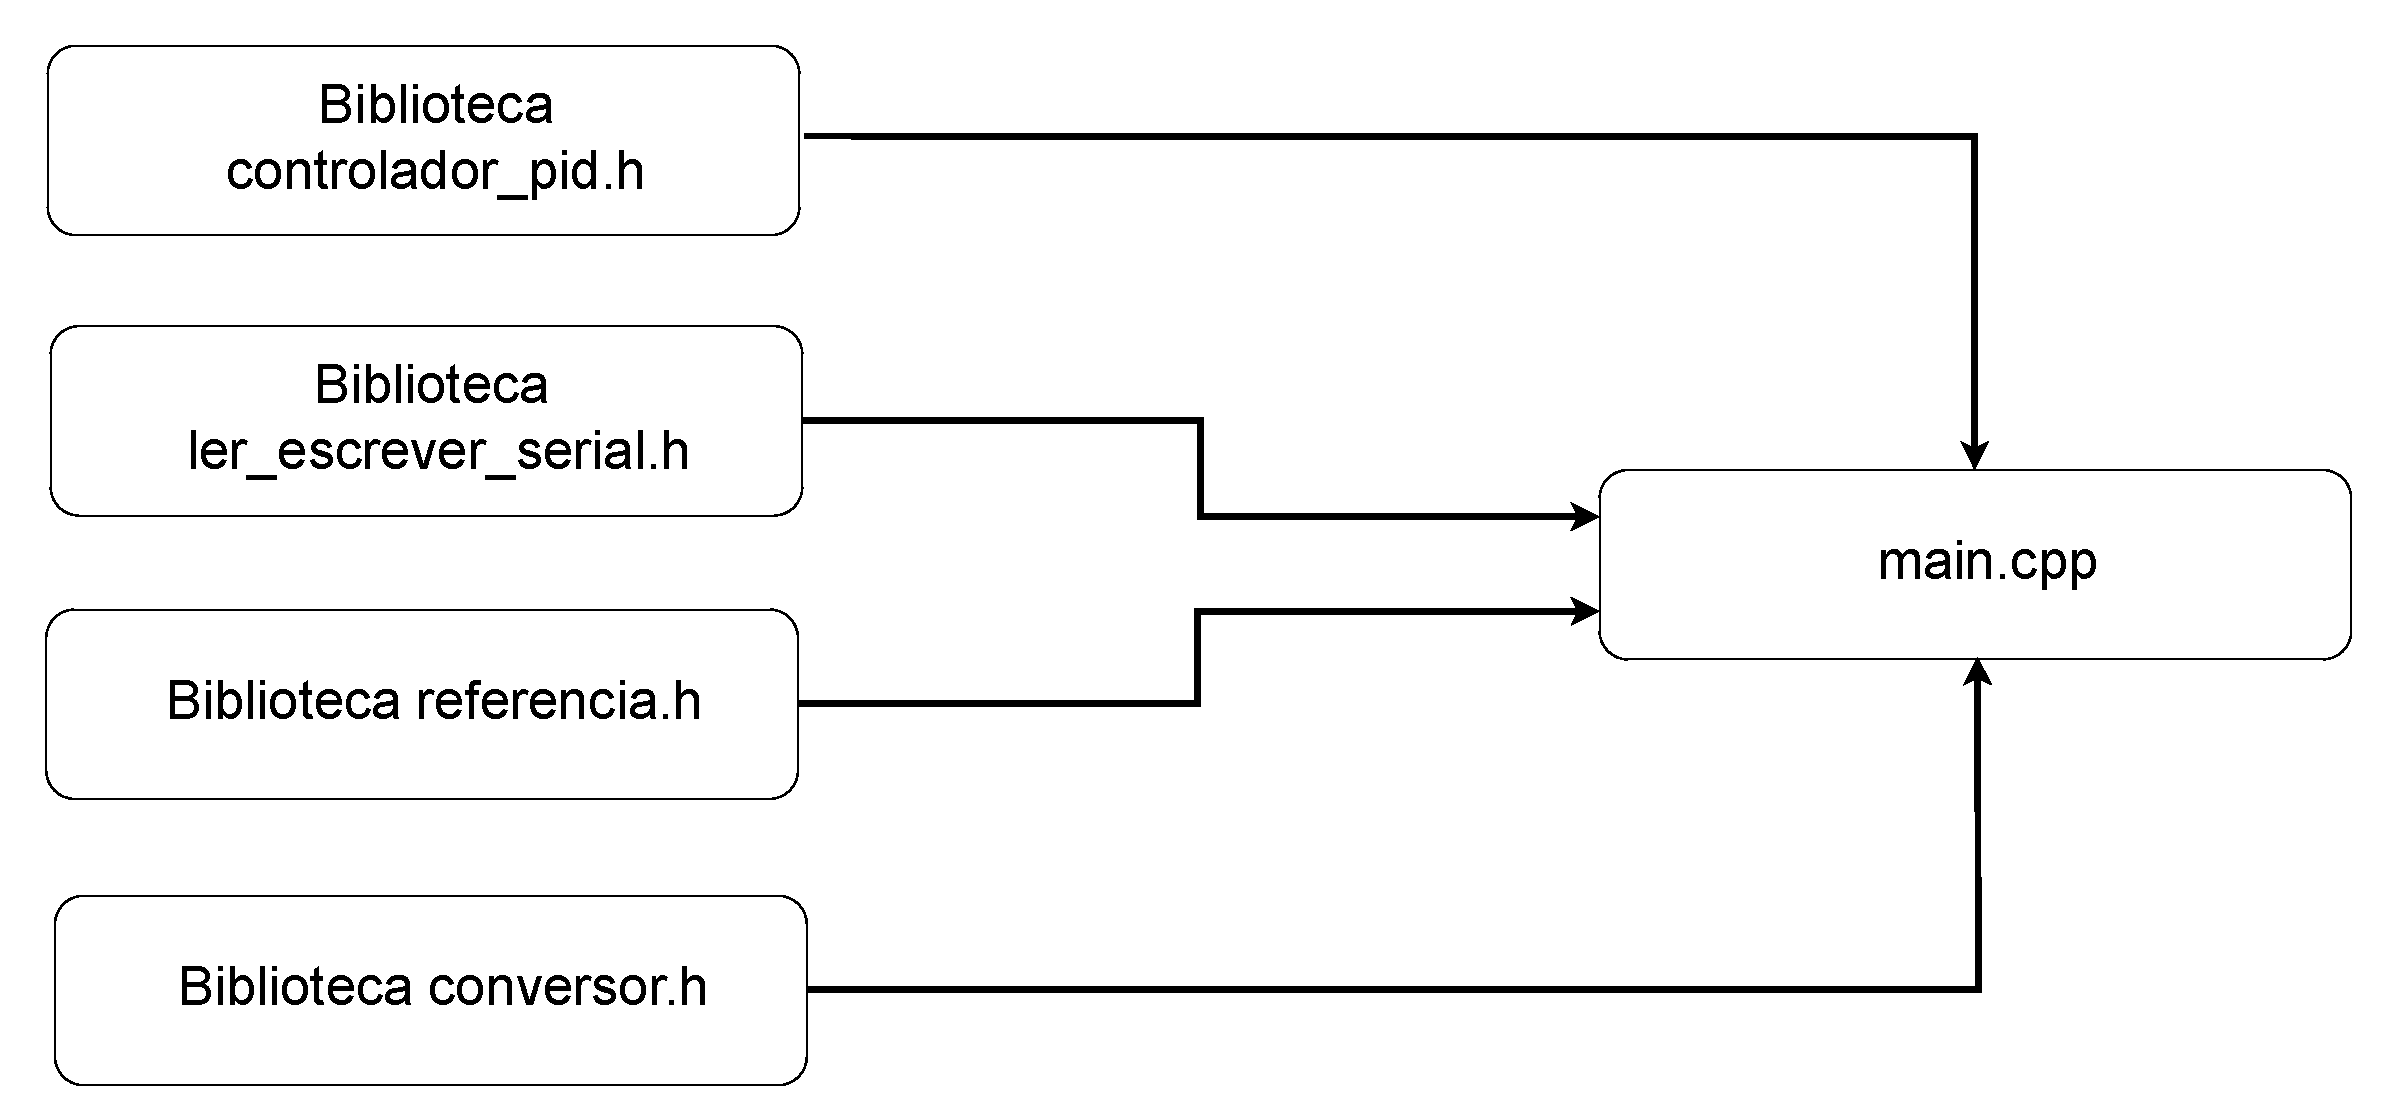
\includegraphics[width=0.8\textwidth]{Capitulos/3_hardware_softwares/3_figuras/arquitetura_firmware.pdf}}
	\caption*{Fonte: elaborado pelo autor (2023).}
	\label{fig3:image_16}
\end{figure}


\subsubsection{Biblioteca ler\_escrever\_serial}

Para realizar a configuração dos parâmetros do sinal de referência em tempo real e o envio dos sinais do sistema via porta serial foi desenvolvido a biblioteca ler\_escrever\_serial, assim, a parte de recebimento e envio de dados do sistema fica centralizada permitindo sua melhoria e modificação sem interferir na lógica do código principal "main.cpp".

\subsubsection{Biblioteca referencia}

O sistema em malha fechada possui uma entrada de referência que o controlador tem por finalidade rastrear, para tornar o projeto do firmware mais legível criou-se o módulo referencia.h em que implementa inicialmente três sinais de referência com a possibilidade de configurar os parâmetros de Amplitude, frequência e offset, sendo esses sinais Onda Quadrada, Onda Senoidal e Onda Dente de Serra. Caso, observe-se a necessidade de outros sinais, basta adicionar a biblioteca.

\subsubsection{Biblioteca conversor}


Essa biblioteca possui uma classe cpp com métodos de conversões de diferentes grandezas, a primeira conversão é do sinal de um potenciômetro para angulo, o segundo método converte o sinal de controle para ciclos PWM, o terceiro método converte de grau para radiano e o quarto de radiano para grau.

\subsubsection{Biblioteca controlador\_pid}

Essa biblioteca implementa uma classe cpp para o controlador PID para ser empregado no protótipo quando selecionado a opção em malha fechada na interface gráfica.


\subsubsection{Arquivo Principal mian.cpp}

A ferramenta PlatformIO possui uma estrutura que permite a criação de bibliotecas e um arquivo main.cpp que implementa a lógica do algorítimo, com isso é possível incluir as bibliotecas desenvolvidas e criar o algorítimo para o que se deseja.


Ou seja, o firmaware para o projeto possui várias funcionalidades que passam pela implementação do sinal de referência, leitura do sensor potenciômetro, envio e recebimento de dados via porta serial e implementação do controlador.

Por fim, com o firmware finalizado, o envio para o ESP32 é realizado usando o PlatfrmIO que concretiza a compilação e escrita no microcontrolador via porta serial.


\section{Fluxograma do Laboratório Virtual}
\label{flu_lab_virtual}
Dado o caráter multifacetado deste projeto, a compreensão das interações entre seus diversos subsistemas pode apresentar desafios significativos. Com o propósito de simplificar e aprofundar esse processo de compreensão, a figura \ref{fig3:image_17} oferece uma representação visual por meio de um diagrama de blocos que esclarece as dinâmicas entre os distintos subsistemas desenvolvidos. Essa abordagem contribui para facilitar o entendimento holístico do sistema na totalidade, proporcionando um recurso valioso para pesquisadores futuros que desejam explorar e aprimorar este laboratório.


\begin{figure}[!h]
	\centering
	\caption{Diagrama do Laboratório Virtual.}
	\efbox{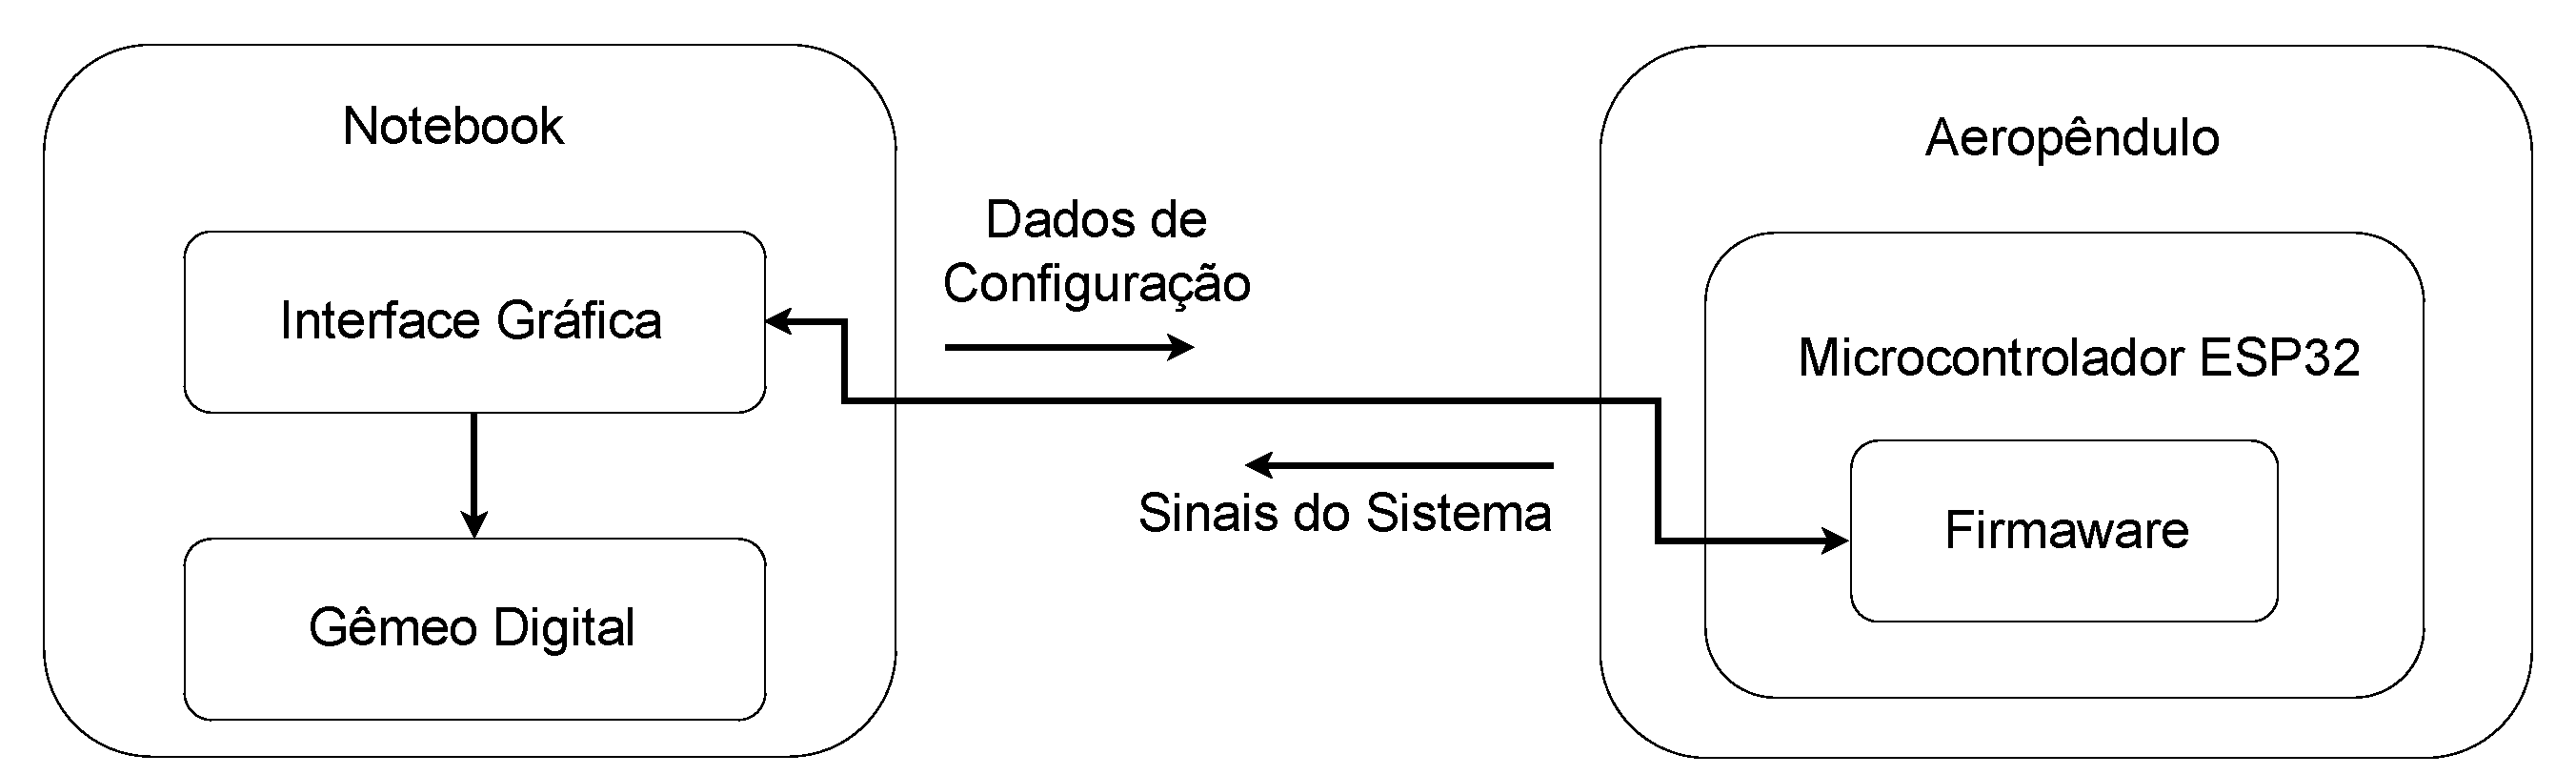
\includegraphics[width=1.0\textwidth]{Capitulos/3_hardware_softwares/3_figuras/diagrama_ecossistema.pdf}}
	\caption*{Fonte: elaborado pelo autor (2023).}
	\label{fig3:image_17}
\end{figure}


